% Trap Streets for Agent Swarms -- arXiv source.
% Build the figures, tables and number macros first:   python -m scripts.build_arxiv     (from the repository root)
% Then compile:   cd arxiv && tectonic main.tex      or      latexmk -pdf main.tex
% Everything in red brackets, \ph{...}, is a placeholder to fill before submission (python -m scripts.arxiv_placeholders lists them).
\documentclass[11pt]{article}

\usepackage[T1]{fontenc}
\usepackage[utf8]{inputenc}
\usepackage{lmodern}
\usepackage[margin=1in]{geometry}
\usepackage{microtype}
\usepackage{amsmath,amssymb,amsthm}
\usepackage{booktabs,array}
\usepackage{graphicx}
\usepackage[dvipsnames]{xcolor}
\usepackage{enumitem}
\usepackage{algorithm}
\usepackage{algpseudocode}
\usepackage[numbers,sort&compress]{natbib}
\usepackage{url}
\usepackage[font=small,labelfont=bf]{caption}
\usepackage[colorlinks=true,linkcolor=blue!50!black,citecolor=blue!50!black,urlcolor=blue!50!black]{hyperref}

\newcolumntype{L}[1]{>{\raggedright\arraybackslash}p{#1}}
\newcolumntype{C}[1]{>{\centering\arraybackslash}p{#1}}
\setlist{itemsep=2pt,topsep=3pt,parsep=0pt}
\setlength{\parskip}{3pt}
\setlength{\emergencystretch}{2em}
\setlength{\parindent}{1.2em}
\renewcommand{\arraystretch}{1.12}

% ---- placeholders and shorthand
\newcommand{\ph}[1]{{\color{red}[#1]}}
\newcommand{\E}{\mathbb{E}}
\renewcommand{\Pr}{\mathbb{P}}
\DeclareMathOperator*{\argmax}{arg\,max}
\newcommand{\Cz}{C_0}
\newcommand{\ie}{i.e.\ }
\newcommand{\eg}{e.g.\ }

\newtheorem{definition}{Definition}
\newtheorem{proposition}{Proposition}
\newtheorem{corollary}{Corollary}
\theoremstyle{remark}
\newtheorem{remark}{Remark}

% generated by scripts/arxiv_tables.py from the result files: do not edit by hand
\newcommand{\nCells}{231}
\newcommand{\nRuns}{7{,}265}
\newcommand{\nFamilies}{8}
\newcommand{\labUSD}{67}
\newcommand{\nAdopters}{2{,}976}
\newcommand{\nBehaviours}{35}
\newcommand{\noCarrier}{56\%}
\newcommand{\bestTop}{16.2\%}
\newcommand{\naiveCalls}{1{,}001}
\newcommand{\trustedCalls}{385}
\newcommand{\crossNaive}{23}
\newcommand{\crossVerified}{3}
\newcommand{\crossRejected}{20}
\newcommand{\avMessages}{173{,}493}
\newcommand{\avPre}{100\%}
\newcommand{\avPost}{97\%}
\newcommand{\avPostMin}{85\%}
\newcommand{\avPostMedian}{98\%}
\newcommand{\avPreWeeks}{47}
\newcommand{\avPostWeeks}{30}
\newcommand{\avPostCopies}{16{,}274}
\newcommand{\avPreCopies}{10{,}880}
\newcommand{\avFirst}{2025-04-02}
\newcommand{\avLast}{2026-09-18}
\newcommand{\benchCells}{150}
\newcommand{\benchAll}{187}
\newcommand{\benchTagsTop}{70.5\%}
\newcommand{\benchEarliestTop}{35.3\%}
\newcommand{\benchLatestTop}{14.6\%}
\newcommand{\benchUniformTop}{11.1\%}
\newcommand{\benchConsTop}{0.8\%}
\newcommand{\benchTagsFA}{6.7\%}
\newcommand{\benchRuleFA}{82.1\%}
\newcommand{\benchConsFA}{6.2\%}
\newcommand{\benchTagsRecall}{72\%}
\newcommand{\benchTagsECE}{0.028}
\newcommand{\liftMin}{$-$1}
\newcommand{\liftMax}{+68}
\newcommand{\nLiftFamilies}{7}
\newcommand{\nLiftTen}{5}
\newcommand{\gatedOpenLo}{25\%}
\newcommand{\gatedOpenHi}{50\%}
\newcommand{\nBypass}{4}
\newcommand{\nBypassWord}{four}
\newcommand{\recheckAfter}{83\%}
\newcommand{\recheckTrace}{8\%}
\newcommand{\recheckEarliest}{9\%}
\newcommand{\recheckFoundLo}{88\%}
\newcommand{\recheckFoundHi}{92\%}
\newcommand{\earlyReach}{80\%}
\newcommand{\earlyEarliest}{80\%}
\newcommand{\qwenEarly}{100\%}
\newcommand{\gptossEarly}{0\%}
\newcommand{\qwenInert}{95\%}
\newcommand{\qwenToken}{100\%}
\newcommand{\glmToken}{9\%}
\newcommand{\stalePerRunLate}{4}
\newcommand{\tauDefault}{100}
\newcommand{\maxAgents}{10}
\newcommand{\gradeA}{90}
\newcommand{\gradeB}{70}
\newcommand{\gradeC}{50}
\newcommand{\gradeD}{25}
\newcommand{\simRescueNaive}{65\%}
\newcommand{\simRescueCal}{1\%}
   % number macros generated from the result files

\title{Trap Streets for Agent Swarms:\\[3pt]\large Making Copying Confess When Reads Go Unlogged}
\author{%
  \ph{Author One}\thanks{\ph{Affiliation, city, country. Email.}} \and
  \ph{Author Two}\thanks{\ph{Affiliation, city, country. Email.}}%
}
\date{\ph{Month Year}}

\begin{document}
\maketitle

\begin{abstract}
\noindent
When many LLM agents share a wiki, notes or memory, one agent's mistake can reach others simply by being copied, and after an incident the operator asks who passed what to whom. We show that ordinary logs usually cannot say: they record what agents wrote, not what they read. In a real shared-wiki incident, even a perfect investigator could name the true source of at most \bestTop{} of copied behaviours, and the obvious detector (``the same string appeared twice'') made \naiveCalls{} copy calls of which only \trustedCalls{} survive base-rate calibration.
We prove ceilings on what any tracer can recover from log content, a bound on false copy calls under monoculture, and soundness of a gateway design in which every served copy carries its own load-bearing token: a \emph{trap street}, after the fictitious streets mapmakers draw to catch copiers. We turn the theory into a traceability audit, the gateway, and a benchmark with a hidden read log.
In \nRuns{} offline agent runs of eight model families, tokens identify the immediate source for \benchTagsTop{} of copying agents against \benchEarliestTop{} for the best simple edit-log rule (false accusations \benchTagsFA{} against \benchRuleFA{}, the latter partly by construction). Whether a token survives depends on whether a model copies links verbatim or re-derives access, so the gain ranges from \liftMin{} to \liftMax{} points. Closing the alternative route raised the traceable share of the \nBypassWord{} models that bypassed tokens from \gatedOpenLo{}--\gatedOpenHi{} to 100\% with no loss of task completion, and tracing a planted bad tip cut the re-check list from \recheckAfter{} to \recheckTrace{} of outputs. We also report what failed: three of our own experiment designs were wrong and one hypothesis we stated in advance was not met.
Code, data and benchmark: \ph{URLs}.
\end{abstract}


\section{Introduction}\label{sec:intro}

Teams of LLM agents increasingly work through shared state: a wiki they edit together, notes and memories they read back later, a chat room, a board of tips~\citep{park2023generative,wu2023autogen}. Shared state is what lets a swarm learn from itself, and it is also how a mistake travels. A wrong fact, a stale configuration, a shortcut that only works by accident, or an injected instruction can be picked up by one agent and passed on to many~\citep{gu2024agentsmith,lee2024prompt}. When that happens, the operator's questions are practical. Where did it enter? Which outputs did it reach, so that those can be re-checked and the rest trusted? And which agents are innocent, so that nobody is blamed or retrained for something they never did?

The records people keep are poorly matched to these questions. A wiki's history says who \emph{wrote} what and when. It does not say who \emph{read} what before acting, and reading is how copying happens in a swarm: an agent is shown a page, picks up a link or a value, and uses it. Without the reads, an investigator can only guess which of several earlier writers an agent learned from. The guess is often wrong, and in a real shared-wiki incident that we analyse, even a \emph{perfect} investigator working from the edit logs could name the true source of at most \bestTop{} of the copied behaviours (Section~\ref{sec:res-real}).

The obvious shortcut is to treat a repeated string as evidence of copying. It misleads for a reason specific to LLM swarms: agents of the same model share habits, so they independently produce the same ``random'' values, field names and URL shapes. In the same incident the shortcut made \naiveCalls{} copy calls, and only \trustedCalls{} of them survive a base-rate calibration; of \crossNaive{} apparent cross-team collusion jumps, \crossVerified{} survive hand verification.

\begin{figure}[t]
\centering
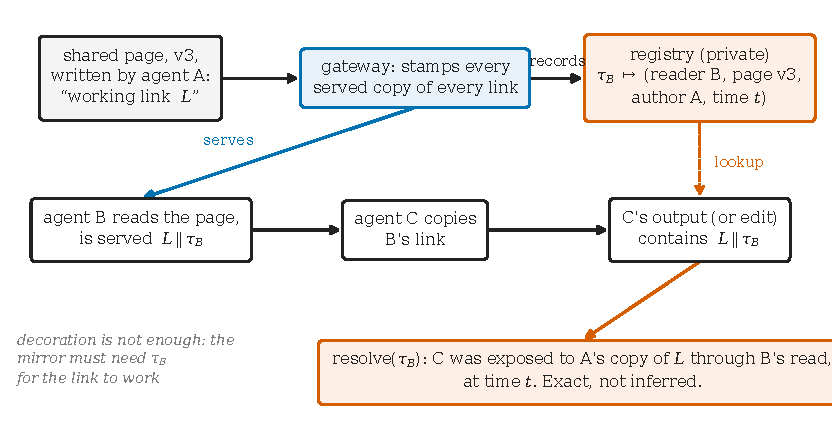
\includegraphics[width=\linewidth]{figures/fig_mechanism.pdf}
\caption{A trap street for a swarm. The gateway serves every copy of every link with its own token $\tau$ and records who was served what. A later copy of the link carries the token, and resolving it names the exact copy it came from. The token must be needed for the link to work: decoration that a copier can drop is not enough (Sections~\ref{sec:res-survival} and~\ref{sec:res-gate}).}
\label{fig:mechanism}
\end{figure}

\paragraph{Trap streets.} Mapmakers have long put a fictitious street on their maps; if it appears on a rival's map, the rival copied~\citep{fictitiousentry}. Security teams plant canary tokens for the same reason~\citep{canarytokens}, and cryptographers trace leaks by giving each recipient a different copy~\citep{chor1994tracing}. We bring the idea to agent swarms. A gateway serves each read of a shared artifact with a token unique to that served copy and the reader, and a registry remembers who was served what. If an agent later copies the link, the token travels with it and names the copy (Figure~\ref{fig:mechanism}). The design questions are the ones the theory and the experiments answer: what can logs alone recover, how should copying be called without being fooled by shared habits, when does a token survive, and what does it cost to make the token unavoidable?

\paragraph{Contributions.}
\begin{enumerate}[leftmargin=1.6em]
  \item \textbf{A measurement of the limits of edit logs} on a real incident and on a second real swarm (AI Village), including a calibrated separation of copying from coincidence (Section~\ref{sec:res-real}).
  \item \textbf{Theory.} Six propositions with proofs: a ceiling on attribution from log content, the value of logging reads and of surviving tokens, a bound on false copy calls that holds under monoculture, soundness of a gateway design, and how trace recall decays with cascade depth (Section~\ref{sec:theory}, Appendix~\ref{app:proofs}).
  \item \textbf{A system and a benchmark.} A traceability audit, a canary gateway, a re-check-list procedure, a local viewer, and a benchmark with a hidden read log and a standard-library scorer (Section~\ref{sec:system}, Appendix~\ref{app:bench}).
  \item \textbf{A lab study with hypotheses stated in advance} of \nRuns{} offline agent runs across eight model families (Section~\ref{sec:setup}), with results on token survival, attribution, bad-tip spread, and the cost of closing the other way in (Section~\ref{sec:results}).
  \item \textbf{A candid account of what went wrong}, and guidance for people who run swarms (Sections~\ref{sec:problems} and~\ref{sec:guidance}).
\end{enumerate}

\paragraph{Findings in brief.}
(i)~Edit logs cap traceability at \bestTop{} in the real incident, while a shared chat that everyone reads is traceable \avPre{} of the time before rooms and \avPost{} after (every week of \avMessages{} messages). (ii)~Calibration removes most naive copy calls. (iii)~On the benchmark, a token identifies the immediate source of \benchTagsTop{} of copying agents against \benchEarliestTop{} for the best simple edit-log rule, with \benchTagsFA{} false accusations against \benchRuleFA{}. (iv)~The gain depends on the model: \liftMin{} to \liftMax{} points, in proportion to how often the token survives copying, because some models re-derive access instead of copying links. (v)~Making the token the only way in lifts the traceable share of the models that bypassed it from \gatedOpenLo{}--\gatedOpenHi{} to 100\%, at no cost in completion. (vi)~After a bad tip, following the trace shrinks the re-check list from \recheckAfter{} of outputs to \recheckTrace{}, but a tip that is there from the start reaches \earlyReach{} of outputs and no list helps much: the saving is in catching a tip early.

The rest of the paper is organised as follows. Section~\ref{sec:related} places the work among related efforts. Section~\ref{sec:problem} defines the problem, Section~\ref{sec:theory} gives the theory, and Section~\ref{sec:system} the system. Section~\ref{sec:setup} states the experiments and the criteria we ran under, Section~\ref{sec:results} reports results, and Sections~\ref{sec:problems}--\ref{sec:guidance} cover problems, limits, ethics and guidance.

\section{Related work}\label{sec:related}

\paragraph{Failure attribution in multi-agent LLM systems.}
A growing line of work asks which agent, and at which step, caused a task to fail, given the log of one multi-agent run. Who\&When~\citep{zhang2025which} introduced a benchmark and studied LLM judges for the task; AgenTracer~\citep{zhang2025agentracer} trains a model to attribute failures; hierarchical and consensus-based approaches improve step-level accuracy~\citep{banerjee2025where}; and FALAT~\citep{rafi2026falat} frames attribution as a dependency-guided search over decisions, tool outputs and messages. These methods assume that the trajectory is recorded in full and ask about one failing run. Our setting differs in two ways: we ask how an item \emph{spread} among many agents through shared state, and the thing that links agents, a read, is exactly what is missing from the log.

\paragraph{Provenance and information-flow tracking.}
Data provenance~\citep{buneman2001why} and information-flow control~\citep{denning1976lattice,enck2010taintdroid} track how data moves through a system that is instrumented to follow it. For LLM agents, recent work tracks information flow through contexts, tool calls and memory~\citep{cai2026ghost}, and a survey organises evidence tracing and execution provenance for agents~\citep{wang2026traces}. Instrumentation is the right answer when the operator controls the data path. Our contribution sits on both sides of that line: an audit that says how much can be recovered when nothing was instrumented, calibrated against the coincidences that shared model habits create, and a gateway design whose tokens make the instrumentation survive being copied by an agent that is free to rewrite the text.

\paragraph{Planted markers.}
Fictitious map entries~\citep{fictitiousentry}, canary tokens~\citep{canarytokens} and traitor tracing~\citep{chor1994tracing} all plant a recipient-specific mark and read it back from a leak. For agents, canary-style protocols have been used to trace an agent back to its owner~\citep{chocron2026owns}, and keyed signals in a model's token distribution to audit which agent produced a text~\citep{nian2026final}. These identify who \emph{produced} an output. We use the same family of ideas to identify which \emph{served copy} an agent was exposed to, which is the quantity that matters when a mistake spreads through shared artifacts, and we study empirically when such a mark survives an LLM's tendency to copy links verbatim or to re-derive them.

\paragraph{Contagion and source inference.}
Locating the source of a rumour or a cascade from partial observations is a classical problem~\citep{shah2011rumors,gomezrodriguez2010inferring}. Those methods assume that the spread is observed through a graph or through activation times. In a swarm that shares artifacts, what is observed are edits, the graph is the unobserved reads, and the ceiling on what is recoverable is a function of what is logged (Section~\ref{sec:theory}).

\paragraph{Mistakes and attacks that spread among agents.}
Infectious jailbreaks and prompt infection show that a single poisoned input can propagate through a population of agents~\citep{gu2024agentsmith,lee2024prompt}, which is why post-incident tracing matters for safety as well as for debugging.

\paragraph{Shared habits.}
Models trained on similar data make similar choices, a form of algorithmic monoculture~\citep{kleinberg2021algorithmic}. For tracing, monoculture is the reason a repeated value is weak evidence of copying, and Proposition~\ref{prop:calib} bounds the cost of ignoring it.

\paragraph{Position.}
To our knowledge no earlier study measures, on real multi-agent logs and in a controlled lab, how much copying between agents is traceable when reads are not logged, calibrates copy calls against shared habits, and evaluates a tracing token across model families with a hidden read log as ground truth. We have searched but not exhaustively; related work may exist that we have missed.

\section{Problem formulation}\label{sec:problem}

\paragraph{Swarm and artifacts.}
A swarm is a set $\mathcal{A}$ of agents that act over time on a set of shared \emph{artifacts} (wiki pages, notes, memory entries, chat rooms) and produce \emph{outputs} (a value, a link, a patch). An artifact has versions; a version is a sequence of \emph{chunks}, each written by one agent. A \emph{reader} that opens an artifact is \emph{served} a copy of its current version.

\paragraph{Logs.}
The \emph{edit log} $E$ holds one record per write or output: (agent, time, channel, content), where the channel is the room, page or thread in which the record is visible. The \emph{read log} $\mathcal{R}$, when it exists, holds one record per served item: (reader, time, channel, the exact content served, the author of the chunk it came from). Most deployments keep $E$ and not $\mathcal{R}$. A \emph{registry} (Section~\ref{sec:system}) is a third, optional record kept by a gateway.

\begin{definition}[Exposure copy and source]\label{def:copy}
Agent $a$ \emph{copies} an item $u$ from agent $b$ if $a$ was served a copy of $u$ whose chunk was written by $b$ before $a$ first used $u$. The \emph{immediate source} of $a$'s use of $u$ is the author of the served copy it used. An agent that used $u$ without having been served it \emph{worked alone}.
\end{definition}
This is the standard exposure notion in contagion studies: it says nothing about intent, and it is what an operator can act on (the agent saw the item). Where several served copies are byte-identical, the immediate source is not determined by the text alone; we return to this in Section~\ref{sec:setup}.

\begin{definition}[Tracer and scores]\label{def:tracer}
A \emph{tracer} maps the logs it is allowed to see to a prediction for each agent: an earlier agent as source, or ``independent''. On a set of agents with known truth, the \emph{top-1 accuracy} is the share of copying agents whose source is named correctly; \emph{recall} is the share of copying agents accused of copying at all; the \emph{false-accusation rate} is the share of agents that worked alone but were blamed on someone. The \emph{predicted spread graph} is the graph of predicted sources.
\end{definition}

\begin{definition}[Carrier coverage]\label{def:coverage}
For a copy event, its \emph{carrier} is an earlier user of the same distinctive item that is visible in the log in the channel where the copy happens. \emph{Carrier coverage} is the share of copy events that have at least one visible carrier. It measures how much of the propagation channel the log shows, and is the audit's headline.
\end{definition}

\begin{definition}[Re-check set]\label{def:recheck}
Given a bad item entering through agent (or post) $o$, the \emph{affected} outputs are those whose chain of copying leads back to $o$. A \emph{re-check set} is a list of outputs predicted to be affected. It is scored by its \emph{size} as a share of all outputs (the work), by \emph{recall} of the affected outputs, and by \emph{precision}.
\end{definition}

\paragraph{What we assume.}
(A1)~Logs are honest: agents do not tamper with the edit log. (A2)~Agents do not deliberately strip or forge tokens; we study what \emph{unintended} copying does to them (Section~\ref{sec:limits}). (A3)~The operator controls the gateway and the shared artifacts, but not what the agents' models do with them. We do not model adversarial agents.

\paragraph{The questions.}
(Q1)~How much of the copying in a real swarm can \emph{any} tracer recover from $E$ alone? (Q2)~How should copying be called without being fooled by shared habits? (Q3)~If an operator can change how artifacts are served, what should be changed and how well does it work across models? (Q4)~After a bad item spreads, what has to be re-checked?

\section{Theory: what logs can and cannot recover}\label{sec:theory}

This section states what can be recovered, how to call copying without being fooled, and what a gateway guarantees. Proofs are short; Appendix~\ref{app:proofs} spells out the assumptions. Throughout, $S$ is the (unknown) immediate source of an adopting agent, $L$ is everything the tracer is allowed to see for that agent, and $\pi_s(L)=\Pr[S=s\mid L]$ is the posterior over earlier agents $s$.

\begin{proposition}[Ceiling]\label{prop:ceiling}
For any tracer, $\Pr[\hat S(L)=S]\le \E\big[\max_s \pi_s(L)\big]$, with equality for the maximum-a-posteriori tracer. The expectation is over the copy process and the logging process.
\end{proposition}
\begin{proof}
Given $L$, a tracer's guess $\hat S(L)$ is independent of $S$, so $\Pr[\hat S=S\mid L]=\pi_{\hat S(L)}(L)\le\max_s\pi_s(L)$. Take expectations over $L$; the bound is attained by choosing an $\arg\max$.
\end{proof}
\begin{corollary}[Identical posts]\label{cor:uniform}
If an adopter chose uniformly among $m$ earlier posts that the log cannot tell apart, then $\pi_s=1/m$ and the ceiling is $\E[1/m]$ over adopters.
\end{corollary}
Corollary~\ref{cor:uniform} is the no-habit case. A tracer that knows copiers' habits (they take the first link, or the newest) can exceed it, and the benchmark metric defined from it (Appendix~\ref{app:bench}) is therefore not an upper bound for such tracers. The ceiling is a property of the \emph{log and the copy process}, not of the tracer: no better tracer can exist, so ``untraceable from these logs'' is a finding.

\begin{proposition}[Reads]\label{prop:reads}
Let $\Cz$ be the ceiling of Proposition~\ref{prop:ceiling} from the edit log alone. Suppose the item-level read is logged for a random share $\rho$ of adoptions, independently of the source chosen, and a logged read identifies the served copy. Then the ceiling is $\rho+(1-\rho)\Cz$.
\end{proposition}
\begin{proof}
Condition on whether an adoption's read is logged. Logged adoptions are identified exactly (accuracy 1). For unlogged ones, independence means the tracer faces the original problem, with best accuracy $\Cz$. Weight by $\rho$ and $1-\rho$.
\end{proof}
A read that names the page but not the item helps much less: in our simulator, logging the page for every copy lifts the ceiling from $0.46$ only to $0.57$, so the recommendation is to log the \emph{item} that was read (Table~\ref{tab:sim} and Section~\ref{sec:res-sim}).

\begin{proposition}[Tokens]\label{prop:tags}
Suppose each served copy of a link carries a token unique to that copy (a \emph{version-unique} token) and a registry maps it to the served copy. If an adopter's output reveals a token with probability $s$, independently of the source chosen, the ceiling is $s+(1-s)\Cz$. If tokens name an \emph{origin} (one token per original item) or a \emph{page}, a revealed token only narrows the candidates to the origin's writers or the page's writers; the ceiling is then $s\,\E[\max_s\pi_s(L,T)]+(1-s)\Cz$, which is below $s+(1-s)\Cz$ unless every origin or page has a single candidate.
\end{proposition}
\begin{proof}
A revealed version-unique token resolves to one served copy, hence to its author, so those adoptions are identified exactly; the rest are as in Proposition~\ref{prop:reads} with $\rho=s$. For an origin or page token, apply Proposition~\ref{prop:ceiling} to the log enlarged by the token.
\end{proof}
The proposition predicts that the gain from tokens is proportional to the survival rate $s$ and to the headroom $1-\Cz$. Section~\ref{sec:res-attr} tests exactly this, and Section~\ref{sec:res-sim} confirms the formula to within $0.008$ in a simulator.

\begin{proposition}[Calibration]\label{prop:calib}
Let independent agents each choose a value of an attribute (a URL parameter, a field name, an identifier) from the same distribution $p$ over values; $p_v$ is the base rate of $v$ and $c=\sum_v p_v^2$ is the collision probability. A \emph{naive} detector flags two agents as copying when they chose the same value. A \emph{calibrated} detector with threshold $\tau>1$ flags them only if they chose the same $v$ and $p_v\le 1/\tau$, \ie when the likelihood ratio of ``copied'' to ``independent'', $1/p_v$, is at least $\tau$. For two independent agents,
\[
\Pr[\text{naive flags}]=c,\qquad \Pr[\text{calibrated flags}]=\sum_{v:\,p_v\le 1/\tau}p_v^2\ \le\ \frac1\tau .
\]
\end{proposition}
\begin{proof}
Both agents choose $v$ with probability $p_v^2$, so the naive rate is $\sum_v p_v^2$. For the calibrated rate, $\sum_{p_v\le1/\tau}p_v^2\le\frac1\tau\sum_{p_v\le 1/\tau}p_v\le\frac1\tau$.
\end{proof}
Monoculture, the tendency of agents of the same model to choose alike, drives $c$ towards $1$ and the naive false-call rate with it, while the calibrated rate stays below $1/\tau$ whatever $c$ is. The price is recall: copying that rides on a common value cannot be told from coincidence and is declined. The bound is per pair; testing $k$ attributes multiplies it by at most $k$ (union bound), and base rates must be estimated, which we do from agents that were first to choose in their structure (Section~\ref{sec:setup}). Figure~\ref{fig:calibration} shows the behaviour in a simulator.

\begin{proposition}[Gateway soundness]\label{prop:gate}
Let a gateway $G$ serve every shared artifact. For each serving (reader $r$, artifact version $v$, chunk $i$, time $t$) it mints a fresh unguessable token $\tau$, embeds it in each link of that chunk, and records $R[\tau]=(r,v,i,\mathrm{author}_i,t)$. Resource servers accept a request only if it carries some $\tau\in\mathrm{dom}(R)$, and tokens are issued only by serving. Then: (a)~every accepted request resolves to exactly one served copy; (b)~if an agent's output reports the request it made, resolving the token in it names the copy the agent was served, hence the author of the chunk it came from, exactly; (c)~for outputs that report the request they made, the survival probability in Proposition~\ref{prop:tags} is $s=1$, so the ceiling is $1$ for the portion of adoptions that go through the gate. Facts an agent learns from a served copy and uses without a gated request are not covered, and an agent that reports a different link from the one it used is attributed to the link it reported.
\end{proposition}
\begin{proof}
(a) Tokens are fresh and recorded once, so $R$ is a function. (b) An accepted request carries some $\tau\in\mathrm{dom}(R)$; because tokens are issued only by serving and re-minted at every serving, $\tau$ was minted for this reader's read of that chunk. (c) A gated output that reports its request reports its token. The restriction in the last sentence is a limit of the design, not of the proof: the gate traces access, not ideas.
\end{proof}

\begin{proposition}[Depth]\label{prop:depth}
Suppose each copy edge of a cascade is recovered independently with probability $q$, and an output at depth $d$ is found by the trace only if all $d$ edges on its path are recovered. The recall of the affected set is $\E[q^{d}]\ge q^{\E[d]}$.
\end{proposition}
\begin{proof}
The probability of recovering a depth-$d$ path is $q^d$; $d\mapsto q^d$ is convex for $q\in(0,1)$, so Jensen's inequality gives the bound.
\end{proof}
This single-path model is pessimistic where an output has several routes to the origin, but it explains two observations: deep cascades are hard to trace from partial evidence (\eg with $q=0.9$, seven hops leave recall $0.9^7\approx0.48$), and a fallback rule that raises $q$ where a token was lost raises recall (Section~\ref{sec:res-tip}).

\paragraph{What the propositions say in practice.}
(1)~Log the \emph{item} read, not only the page; each logged share $\rho$ is worth $\rho(1-\Cz)$. (2)~A token is worth its survival rate. (3)~Call copying only against a base rate, and accept the recall that costs. (4)~A gateway that makes the token needed moves $s$ towards $1$ for gated outputs. (5)~Per-edge recovery must be high, or a fallback present, for deep cascades.

\section{System}\label{sec:system}

\subsection{Overview}
Figure~\ref{fig:architecture} shows the components. A \emph{gateway} sits between the agents and the shared artifacts and tools; it stamps every served copy and keeps a registry. The edit log (and, when available, the read log and the registry) feed an \emph{audit} that calls copies, links reads to uses, and produces a \emph{trace graph} with an evidence tier on every edge. The graph yields an attribution for each output and a re-check list. A \emph{benchmark harness} runs swarms in a sandbox, keeps the hidden read log as the answer key, and scores any tracer that sees only what a real investigator would. A local \emph{viewer} draws the trace graph as an ant colony for human inspection. Every component except the gateway works on logs that already exist.

\begin{figure}[t]
\centering
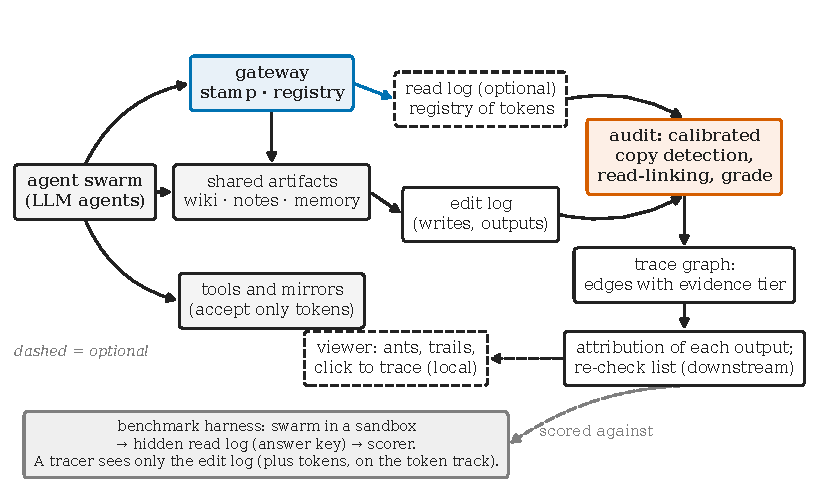
\includegraphics[width=\linewidth]{figures/fig_architecture.pdf}
\caption{Components and data flow. Dashed boxes are optional: the audit works on the edit log alone, and uses the read log and the registry when they exist. The benchmark harness scores a tracer against the hidden read log.}
\label{fig:architecture}
\end{figure}

\subsection{The audit: calibrated copy detection}\label{sec:audit}
The audit takes a log with fields agent, time, channel and content (other shapes are mapped to these) and answers: if something bad spread through this swarm, could it be traced? Algorithm~\ref{alg:audit} extracts distinctive strings, calls copies only where a string is strong evidence, and reports carrier coverage (Definition~\ref{def:coverage}).

\begin{algorithm}[t]
\caption{Calibrated copy detection}\label{alg:audit}
\begin{algorithmic}[1]
\Require events $E$ sorted by time, each $(a,t,c,x)$ = (agent, time, channel, content); $N_{\max}=\maxAgents{}$
\State $\mathrm{first}\gets$ empty map: token $\mapsto$ agent $\mapsto (t,c)$
\For{each event $(a,t,c,x)$ in $E$}
  \For{each $w\in\textsc{Tokens}(x)$}
    \State \textbf{if} $a\notin\mathrm{first}[w]$ \textbf{then} $\mathrm{first}[w][a]\gets(t,c)$
  \EndFor
\EndFor
\For{each token $w$ with $|\mathrm{first}[w]|\ge2$}
  \State $(\kappa,\sigma)\gets\textsc{Classify}(w)$;\quad order its users by first-use time as $u_1,u_2,\dots,u_n$
  \State $\mathrm{trusted}\gets n\le N_{\max}\ \wedge\ \kappa\notin V\ \wedge\ (\sigma=\text{high}\ \vee\ n\le3)$
  \For{$k=2,\dots,n$}
    \State $\mathrm{carriers}\gets\{u_j:\ j<k,\ \mathrm{channel}(u_j)=\mathrm{channel}(u_k)\}$
    \State emit $(w,u_k,\mathrm{carriers},\mathrm{trusted})$
  \EndFor
\EndFor
\State $\mathrm{coverage}\gets\big|\{\text{trusted rows with carriers}\}\big|\,/\,\big|\{\text{trusted rows}\}\big|$; grade by Table~\ref{tab:grade}
\end{algorithmic}
\end{algorithm}

\textsc{Tokens} are runs of at least 12 characters from $[\mathrm{A\text{-}Za\text{-}z0\text{-}9\_\text{-}}]$ after URL-decoding up to three times and removing redaction markers, kept only if they are not common words or headers, not long hex or digit runs, have at least seven distinct characters, and contain a digit, mixed case or an underscore. \textsc{Classify} labels a token as a UUID, a high-entropy identifier (Shannon entropy at least $3.3$ bits per character), a timestamp, a snake\_case or camelCase identifier, or other; $V$ is the set of vocabulary classes (snake\_case and camelCase identifiers and round, constructed timestamps), which agents type independently and which are never trusted. A string is \emph{trusted} when it is used by at most $N_{\max}=\maxAgents{}$ agents, is not vocabulary, and is either strong evidence (a UUID or minted identifier) or used by at most three agents. This is the practical counterpart of the base-rate test of Proposition~\ref{prop:calib}; Section~\ref{sec:res-real} uses the explicit likelihood-ratio test on the real incident. The audit also reports the \emph{best possible top-1} (Corollary~\ref{cor:uniform}), the strings that many agents type (``everyone types this''), naive against calibrated counts, and what to log next. When no trusted copy exists it reports N/A rather than a grade: a log in which agents share nothing distinctive proves nothing about traceability.

\begin{table}[t]
\centering\small
\caption{Grade thresholds on carrier coverage (Definition~\ref{def:coverage}).}\label{tab:grade}
\begin{tabular}{@{}lccccc@{}}
\toprule Grade & A & B & C & D & F \\ \midrule coverage $\ge$ & \gradeA\% & \gradeB\% & \gradeC\% & \gradeD\% & below \\ \bottomrule
\end{tabular}
\end{table}

The audit runs as a command-line tool and as a browser page that reads the file locally and sends nothing anywhere; a parity test requires the two to agree on counts, grade and shared-string tables on all test files, including samples of real logs.

\subsection{Linking reads to uses}\label{sec:links}
If the log has read events, Algorithm~\ref{alg:links} links an agent's first later event that contains something it read to the author of what it read. The most specific matching read wins, so a short tagless link inside a longer tagged one is not a second candidate. If no exact copy matches, the \emph{weak} tier matches the same link with its tag, token or query stripped: the agent used what it read, but not the copy it was served, so which copy is unknown. The tiers are reported separately because they carry different evidence.

\begin{algorithm}[t]
\caption{Read-linking}\label{alg:links}
\begin{algorithmic}[1]
\Require sorted events; read events carry (reader, time, served content, source author)
\For{each agent $a$ and its first non-read event $e$ that contains something $a$ read earlier}
  \State $H\gets\{r\in\mathrm{reads}_a\text{ before }e:\ |r.\mathrm{content}|\ge12,\ r.\mathrm{source}\ne a,\ r.\mathrm{content}\subseteq e.\mathrm{content}\}$
  \If{$H\ne\emptyset$} \State remove from $H$ every $r$ whose content is a proper substring of another member's content;\ $\mathrm{weak}\gets\textbf{false}$
  \Else \State $H\gets\{r:\ \textsc{Strip}(r.\mathrm{content})\subseteq\textsc{Strip}(e.\mathrm{content})\}$;\ $\mathrm{weak}\gets\textbf{true}$
  \EndIf
  \If{$H\ne\emptyset$} \State $\mathrm{sources}\gets$ distinct authors in $H$;\ emit $(a,\mathrm{sources},\ \mathrm{exact}=(|\mathrm{sources}|=1\wedge\neg\mathrm{weak}),\ \mathrm{weak})$
  \EndIf
\EndFor
\end{algorithmic}
\end{algorithm}

\subsection{The canary gateway}\label{sec:gateway}
Algorithm~\ref{alg:gate} is the gateway of Proposition~\ref{prop:gate}. The design space has two axes. \emph{Granularity}: a token per served copy (version-unique), per origin, or per page; Proposition~\ref{prop:tags} says only the first identifies the immediate source. \emph{Necessity}: an \emph{inert} tag is decoration (a query parameter the mirror ignores) that a copier can drop without penalty; a \emph{load-bearing} token is part of what the link needs to work (a session segment the mirror requires). Section~\ref{sec:res-survival} shows that necessity matters and that it matters differently for different models. In the lab, the inert condition appends a random-looking query value to every served link, and the load-bearing condition re-mints a fresh valid session token in every served link. A gateway also needs \emph{closure}: if the resource server hands a session to anyone who asks, an agent can bypass the token; the gated condition removes that route (Section~\ref{sec:res-gate}).

\begin{algorithm}[t]
\caption{Canary gateway}\label{alg:gate}
\begin{algorithmic}[1]
\Procedure{Serve}{reader $r$, version $v$, time $t$}
  \For{each chunk $i$ of $v$ and each link $\ell$ in chunk $i$}
    \State $\tau\gets$ fresh random token;\quad $R[\tau]\gets(r,v,i,\mathrm{author}_i,t)$
    \State replace any token already in $\ell$ by $\tau$ \Comment{a copied token is never reused}
  \EndFor
  \State \Return the stamped text
\EndProcedure
\Procedure{Accept}{request $q$}
  \State $\tau\gets\textsc{TokenIn}(q)$;\quad \textbf{if} $\tau\in\mathrm{dom}(R)$ \textbf{then forward} $q$ \textbf{else refuse}
\EndProcedure
\Procedure{Resolve}{$\tau$} \State \Return $R[\tau]$ \EndProcedure
\end{algorithmic}
\end{algorithm}

\subsection{Re-check sets}\label{sec:recheck}
Given an origin $o$, Algorithm~\ref{alg:recheck} follows trace edges forward and returns the downstream set. Edges from hidden sources and from coincidences are not followed, so the list never relies on a guess; this is conservative where the log is silent. The comparison lists in Section~\ref{sec:res-tip} are: everything after the item appeared, the earliest-writer rule, tokens alone, and tokens with the earliest-writer rule as the fallback where a token was lost.

\begin{algorithm}[t]
\caption{Re-check set (downstream)}\label{alg:recheck}
\begin{algorithmic}[1]
\Require trace edges $(u\to v,\ \mathrm{kind})$ with $\mathrm{kind}\in\{$exact, one-of-several, weak, string-in-room, hidden, coincidence$\}$; origin $o$
\State $\mathrm{out}\gets\emptyset$;\quad queue $\gets[o]$
\While{queue not empty}
  \State pop $u$;\ \textbf{for} each edge $(u\to v,\mathrm{kind})$ with $\mathrm{kind}\notin\{\text{hidden},\text{coincidence}\}$ and $v\notin\mathrm{out}\cup\{o\}$: add $v$ to $\mathrm{out}$ and to the queue
\EndWhile
\State \Return $\mathrm{out}$
\end{algorithmic}
\end{algorithm}

\subsection{Benchmark and viewer}\label{sec:benchsys}
The benchmark exports each lab run in three parts: the \emph{edit-log view} that a real investigator would have, the \emph{hidden truth} (which copy each agent was served), and, for the token track, the \emph{registry}. A standard-library scorer reports the metrics of Definition~\ref{def:tracer} with run-level bootstrap intervals and ships five baselines (Appendix~\ref{app:bench}). The viewer is a local page that runs the same tracing core as the audit and draws each agent as an ant in a chamber for its room, with trails for trace edges; clicking an ant shows its trace back and its downstream set. It makes no network request and masks strings from the log by default.

\paragraph{Cost.} The audit is linear in the number of tokens in the log; read-linking is linear in events times reads per agent; the downstream search is linear in the trace graph. The gateway adds a random token and a registry write per served link.

\section{Experimental setup and criteria}\label{sec:setup}

We use four sources of evidence: two real logs, a simulator with a known answer, and an offline lab of LLM agents in which a hidden read log provides the truth. This section states the criteria each was run under.

\subsection{Real logs}\label{sec:setup-real}
\paragraph{The incident.}
A shared wiki edited by AI agents over a short, intense period, available to us as revision histories (writes), with no record of page views. Dataset access and release terms: \ph{INCIDENT-DATA-CITATION-AND-PERMISSION}. We analyse \nAdopters{} adopters of \nBehaviours{} behaviours (every behaviour with at least 20 named adopters). For a behaviour, a \emph{carrier} of an adopter is an earlier agent who wrote the behaviour's marker string on the same page; best top-1 is the uniform ceiling of Corollary~\ref{cor:uniform}, taken as $0$ for adopters with no visible carrier. Markers are rare strings invented by agents (the wrapper side of a URL, common-knowledge strings blacklisted, the copier's URL required to resemble the source's). The coincidence analysis is restricted to URL parameters known to be inert (cache-busters and dummies), because an early attempt that counted every non-URL parameter was wrong: most such parameters change what is fetched. A \emph{naive copy call} is a reuse of another agent's URL structure carrying an inert value that appeared before; it is \emph{calibrated} when the likelihood ratio $1/p$ is at least \tauDefault{} (Proposition~\ref{prop:calib}), with $p$ estimated from the agents that were first to choose a value in their structure. \emph{Cross-team jumps} are marker copies whose source and copier pages belong to different task families; each was checked by hand for breadth (how many pages and agents use the string), for a nearer same-team carrier, and for whether it is a minted token or vocabulary (field names, round timestamps). No URL was fetched at any point: everything is read from the logged text.

\paragraph{AI Village.}
A long-running multi-agent environment with a shared chat among agents of several vendors~\citep{aidigest2026aivillage}. We use the agent chat, \avMessages{} messages from \avFirst{} to \avLast{}, cut into 7-day windows. Before the launch of chat rooms (2026-02-25) every earlier message is visible to everyone; afterwards, an earlier message counts as visible to an adopter only if the adopter also posted in that room, a generous proxy for room membership, so room-scoped coverage is an upper bound. Markers are rare strings (Algorithm~\ref{alg:audit}) used by two to ten agents; coverage is pooled by copy events, with Wilson intervals~\citep{wilson1927probable}, and the per-week spread uses weeks with at least 100 copy events. We report every week of the dataset; an earlier version of this analysis used four hand-picked weeks and overstated the effect of rooms (Section~\ref{sec:problems}).

\subsection{Simulator}
The simulator generates a swarm with a known copy process: each adopter copies an item from an earlier post chosen by a copy rule (uniform, recency-biased or popularity-biased, plus two rules outside the model family of the model-based tracer: homophily and a hard time window), a share of reads happens off the page where the log cannot see it (25\% or 85\%), and tags survive with probability $s$. We compare tracers (earliest, latest, most similar, a tiered heuristic, and a model-based tracer that learns the copy process from the log by expectation--maximisation) with the exact Bayes ceiling, over 12 seeds with about 3,400 adoptions per cell. It verifies the propositions; it is not evidence about LLM behaviour.

\subsection{The offline lab}\label{sec:setup-lab}
\paragraph{Task and sandbox.}
Every run is offline: all hosts are on the reserved \texttt{.invalid} domain and nothing leaves the sandbox. Agents are told that a data server is down and asked to find one number in a dataset (the median rent of one county) through four public ``reader'' mirrors whose URL formats differ: one works, one needs a percent-encoded URL, one is overloaded, and one serves a stale cached snapshot with an old value unless a query parameter is added (the full prompt is in Appendix~\ref{app:prompt}). In wiki worlds agents also have \texttt{list\_pages}, \texttt{read\_page} and \texttt{write\_page}; they must call \texttt{submit} with the number and the exact URLs that worked, within 16 tool calls (8 in the no-wiki world).

\paragraph{Worlds and tag conditions.}
Table~\ref{tab:design} lists the worlds. W1 is a plain shared wiki. W2 adds a team-notes page where agents are asked to post their working URL, and a planted tip that appears there after five agents have submitted and links to the stale mirror (a link, never the value, so an agent must fetch to learn any number); the stale mirror gives no warning. W2E is W2 with the tip present from the start. W3 mixes all eight families in one wiki. W4 and W4G are the access-control pair of Section~\ref{sec:res-gate}. Three \emph{tag conditions} apply to a world: \emph{none} (links served as written), \emph{inert} (every served link gets a random-looking query value that the mirrors ignore), and \emph{load-bearing} (every served link gets its own session token that the mirrors require, re-minted at every serving).

\paragraph{Swarms and models.}
A swarm is 30 agents of one model unless stated (sizes 10 and 100 in a sweep, 45 for the mixed swarm), five running concurrently, each an independent LLM call loop with the tools above. We use eight open-weight model families through one inference provider~\citep{nebius2026tokenfactory} and a stronger member of the core family for a check; the identifiers are in Table~\ref{tab:models}. A ninth family never produced a structured tool call in the harness and was dropped, and is reported here and not hidden.

\paragraph{Truth and what the tracer sees.}
Truth is the hidden read log: an agent \emph{copied} if it was served a copy of the route it used before it first used it, and its immediate source is the author of the served copy it reproduced exactly (the exact copy is unique when tags are present; otherwise it falls back to the most recent read of that route). An agent's outcome is its first fetch that returned a value, or its submission if it never fetched. Where several posts carry byte-identical links the source is not defined by the text, so attribution accuracy is reported only for tagged conditions; untagged runs are scored by the ceiling and by copy-versus-independent. The tracer sees only the edit log (wiki writes and submissions), plus the registry on the token track.

\paragraph{Baselines and metrics.}
The simple rules blame the latest, the earliest or a random earlier writer of the same link; the \emph{best simple rule} is the best of the three for each run, chosen with the answer key in hand, which is generous to the baseline. The token tracer reads the token where it survived and falls back to the same best rule where it did not; an earlier version fell back to ``latest writer'' and made tokens look harmful for several models, a flaw in the comparison that we fixed (Section~\ref{sec:problems}). Metrics are those of Definitions~\ref{def:tracer} and~\ref{def:recheck}.

\paragraph{Statistics.}
Agents in one swarm read each other and are not independent, so rates are pooled over runs and intervals come from a bootstrap that resamples runs~\citep{efron1979bootstrap} (2,000 resamples; with fewer than three runs the interval is the minimum and maximum over runs).

\paragraph{Hypotheses stated in advance.}
Before the lab runs we wrote down five hypotheses with thresholds (Table~\ref{tab:hyp}). They were fixed in our plan, not registered with an external registry. We report each outcome, including those that failed.

\paragraph{Exclusions, cost and safety.}
\begin{table*}[t]
\centering
\footnotesize
\setlength{\tabcolsep}{4pt}
\caption{The offline lab as it was run (read from the run records). A run is one swarm; ``size'' is agents per swarm.}\label{tab:design}
\begin{tabular}{@{}lL{4.6cm}lL{2.0cm}lrr@{}}
\toprule
World & What it is & Models & Tags & Size & Runs & Agent runs \\
\midrule
FP & no wiki; independent agents; we record the ``random'' values each model adds to a URL & 8 models & none & 30 & 24 & 720 \\
W1 & a shared wiki; agents route around a ``down'' data server and share working links & 8 models & none/\allowbreak inert/\allowbreak load-bearing & 10, 30, 100 & 66 & 2{,}090 \\
W2 & W1 plus a team-notes page; a bad tip appears on it after 5 agents have submitted, and the stale mirror it points to gives no warning & 9 models & none/\allowbreak inert/\allowbreak load-bearing & 30 & 62 & 1{,}860 \\
W2E & like W2, but the bad tip is there from the start & 8 models & none/\allowbreak inert/\allowbreak load-bearing & 30 & 44 & 1{,}320 \\
W3 & like W2, with agents from all eight model families in one wiki & mixed (all 8) & none/\allowbreak inert/\allowbreak load-bearing & 45 & 15 & 675 \\
W4 & a coordinator posts a working link; the mirror still hands a session to anyone, so agents can find their own way in & 5 models & load-bearing & 30 & 10 & 300 \\
W4G & like W4, but the mirror hands out nothing: the only way in is a link the wiki served & 5 models & load-bearing & 30 & 10 & 300 \\
\midrule
All &  &  &  &  & 231 & 7{,}265 \\
\bottomrule
\end{tabular}
\par\smallskip\parbox{0.96\linewidth}{\footnotesize 14 connectivity checks are not counted. Three flawed bad-tip designs were set aside (Section~\ref{sec:problems}); the run records of 2 of them are kept with the data.}
\end{table*}
Connectivity checks (seed 900 and up) are not experiments and are excluded everywhere. Three flawed bad-tip designs were set aside (Section~\ref{sec:problems}); the run records of two of them are kept with the data. The analysed runs cost about \$\labUSD{} in inference under a hard cap enforced by the runner. All tasks are benign and fictional; refusals are logged; nothing was run against anyone's live system.

\section{Results}\label{sec:results}

\subsection{What edit logs recover on real logs}\label{sec:res-real}
\begin{table}[t]
\centering
\small
\caption{Results on two real logs. The incident is a shared wiki edited by AI agents; AI Village is a long-running multi-agent environment with a shared chat.}\label{tab:real}
\begin{tabular}{@{}lp{8.2cm}r@{}}
\toprule
Log & Measurement & Result \\
\midrule
Incident & adopters analysed (35 behaviours, $\geq$20 adopters each) & 2{,}976 \\
Incident & adopters with no visible carrier & 56\% \\
Incident & best possible top-1 source accuracy from the edit log & 16.2\% \\
Incident & naive ``same string'' copy calls $\to$ calls that survive calibration & 1{,}001 $\to$ 385 \\
Incident & cross-team collusion jumps flagged $\to$ verified by hand & 23 $\to$ 3 \\
AI Village, one chat & copies with a visible source (47 weekly windows, 10{,}880 copies) & 100.0\% \\
AI Village, rooms & copies with a visible source (30 weekly windows, 16{,}274 copies) & 97.0\% [96.7--97.2] \\
AI Village, rooms & weekly coverage: lowest / median / highest & 84.9\% / 98.4\% / 100\% \\
\bottomrule
\end{tabular}
\par\smallskip\parbox{0.96\linewidth}{\footnotesize Intervals are 95\% Wilson intervals. Coverage in AI Village is the share of copy events whose earlier author is visible in the log where the copy happened (Section~\ref{sec:setup}).}
\end{table}
In the incident, \noCarrier{} of the adopters had no visible carrier at all, and the best possible top-1 attribution from the edit log, even for a perfect tracer, was \bestTop{} (Table~\ref{tab:real}). The agents were reading from places the log does not record. A weaker, marker-based estimate agrees in direction: the earlier writer of a marker string was visible in 16--20\% of cases.

The same measurement on AI Village gives the opposite picture, for a reason that supports the argument (Figure~\ref{fig:visibility}). Its chat is a channel everyone can read and the log contains it, so before the launch of rooms \avPre{} of copy events had a visible source across \avPreWeeks{} weeks (\avPreCopies{} events), and after it \avPost{} across \avPostWeeks{} weeks (\avPostCopies{} events; lowest week \avPostMin{}, median \avPostMedian{}). The dip after the launch lasted about three weeks (the weeks starting 11, 18 and 25 March 2026: 95\%, 88\% and 85\%) and then recovered. Pre-rooms coverage is close to tautological (a fully shared log shows every earlier message), and the room-scoped figure is an upper bound because it counts a room as visible whenever the adopter posted in it; the claim is directional: traceability is a property of what was logged, and the incident logged edits but not reads.

\begin{figure}[t]
\centering
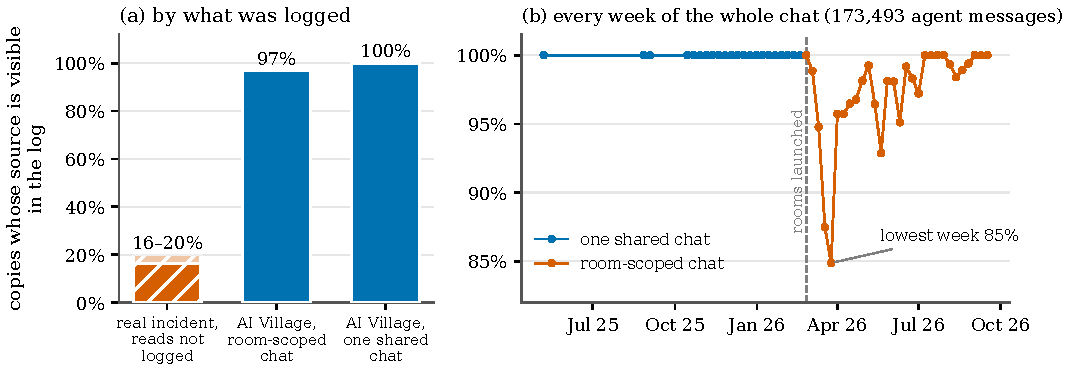
\includegraphics[width=\linewidth]{figures/fig_visibility.pdf}
\caption{Traceability depends on what was logged. (a)~Share of copy events whose source is visible in the log: a real incident with unlogged reads against AI Village chat. (b)~Every week of the whole AI Village chat (weeks with at least 100 copy events); the dashed line marks the launch of chat rooms.}
\label{fig:visibility}
\end{figure}

\subsection{The coincidence trap}\label{sec:res-coincidence}
On the incident, the naive detector made \naiveCalls{} copy calls and \trustedCalls{} survive the likelihood-ratio test at $\tau=\tauDefault{}$ (Figure~\ref{fig:calibration}a); the others rest on values common enough that chance explains them. Of \crossNaive{} apparent cross-team collusion jumps, \crossRejected{} were shared vocabulary that many agents type independently (dataset field names, schema words, round timestamps, one used by 41 agents on 12 pages and another by 49 agents on 60 pages), and \crossVerified{} survived. Those three share a property: each rode on a token minted per fetch (one archived document appears with 48 distinct session-token values, so a specific value cannot be obtained independently), or on an agent-minted short link. In other words, the only provable cross-team copying in the incident was provable because the link carried a unique, needed token: a trap street that occurred by accident, and direct support for the design of Section~\ref{sec:gateway}.

\begin{figure}[t]
\centering
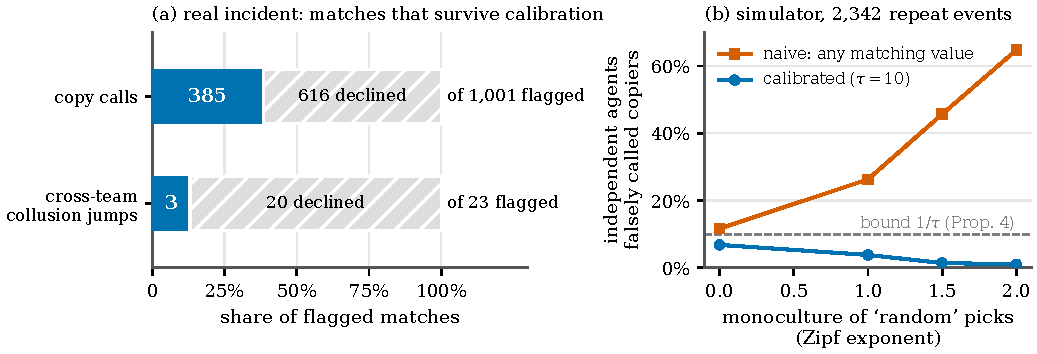
\includegraphics[width=\linewidth]{figures/fig_calibration.pdf}
\caption{The coincidence trap. (a)~On the real incident, most naive copy calls and cross-team collusion jumps do not survive calibration. (b)~In a simulator, the naive detector falsely calls more independent agents copiers as their choices become more alike (monoculture), while the calibrated detector stays below the bound $1/\tau$ of Proposition~\ref{prop:calib} (here $\tau=10$).}
\label{fig:calibration}
\end{figure}

\subsection{The theory against a simulator}\label{sec:res-sim}
\begin{table*}[t]
\centering
\small
\caption{Top-1 accuracy of tracers against the exact Bayes ceiling in a simulator with a known answer (12 seeds, about 3,400 adoptions per cell).}\label{tab:sim}
\begin{tabular}{@{}lcccccc@{}}
\toprule
Copy model & Bayes ceiling & Earliest & Latest & Most similar & Heuristic & Model-based \\
\midrule
uniform & 0.460 & 0.162 & 0.152 & 0.356 & 0.372 & \textbf{0.458} \\
recency-biased & 0.799 & 0.098 & 0.382 & 0.533 & 0.538 & \textbf{0.796} \\
popularity-biased & 0.538 & 0.260 & 0.117 & 0.250 & 0.260 & \textbf{0.511} \\
\bottomrule
\end{tabular}
\par\smallskip\parbox{0.96\linewidth}{\footnotesize The model-based tracer learns the copy process from the log alone. Under three further copy rules, two of them outside the model family it assumes (marked $^{*}$), it keeps 88--101\% of the ceiling (Appendix~\ref{app:tables}).}
\end{table*}
The model-based tracer reaches the exact Bayes ceiling under uniform and recency-biased copying (Table~\ref{tab:sim}; Figure~\ref{fig:simulator}a) and is calibrated (expected calibration error $0.019$~\citep{naeini2015obtaining}: when it reports 90--100\% it is right 98\% of the time; at 50--60\%, 52\%). The simple rules are far below it, and the heuristic collapses when most reads are off the page (Table~\ref{tab:robust} in Appendix~\ref{app:tables}). Proposition~\ref{prop:reads} is matched exactly (with $\Cz=0.46$ and half the reads logged, ceiling $0.727$ predicted and $0.727$ measured), and Proposition~\ref{prop:tags} to within $0.008$ for version-unique tags (Figure~\ref{fig:simulator}b). One tag per origin barely helps ($0.466$--$0.474$), and one tag per page behaves like a page-level read. Page-level reads are a weak substitute for item-level ones: logging the page for every copy lifts the ceiling only from $0.46$ to $0.57$. The simulator and the tracer share a model family, which is why we also test copy rules outside it (marked $^*$ in Table~\ref{tab:robust}): the tracer keeps 88--101\% of the ceiling there.

\begin{figure}[t]
\centering
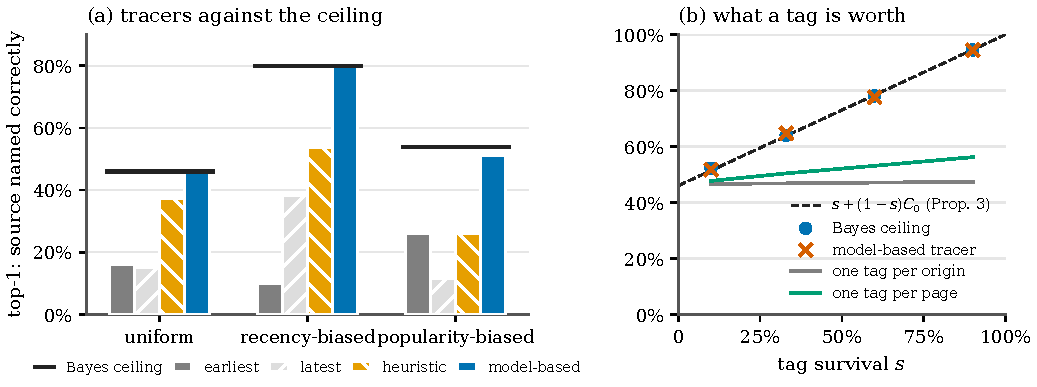
\includegraphics[width=\linewidth]{figures/fig_simulator.pdf}
\caption{The theory against a simulator with a known answer. (a)~Top-1 accuracy of tracers against the exact Bayes ceiling (black bars) under three copy rules. (b)~What a tag is worth: the ceiling and the model-based tracer follow $s+(1-s)\Cz$ for version-unique tags; tags per origin or per page barely help.}
\label{fig:simulator}
\end{figure}

\subsection{Does the token survive copying?}\label{sec:res-survival}
It depends on the model (Figure~\ref{fig:survival}). Models that copy links verbatim carried both decoration and tokens through: the core model kept the inert tag in \qwenInert{} of copies and the token in \qwenToken{}. Models that fetch their own session kept the token in only a minority of copies, \glmToken{} for the weakest, and decoration survived at rates that varied from 4\% to 28\%. Reading transcripts shows why. The core model's typical run is: list pages, read the page, fetch the wiki's link, submit it; the token rides along. The other models read the wiki to learn the \emph{method} and then redo it: they fetch the mirror's root to obtain a session of their own and use that, so the wiki's token is bypassed even though the link needs \emph{a} token, because in this world the mirror hands sessions to anyone. We count these agents as copiers of the behaviour, since they were served the route first, and the token, correctly, does not follow them: \emph{tags trace the artifact, not the idea}. Hypothesis H1 (Table~\ref{tab:hyp}) was therefore not met: no family satisfied both halves, because decoration survived too for the models that copy verbatim.

\begin{figure}[t]
\centering
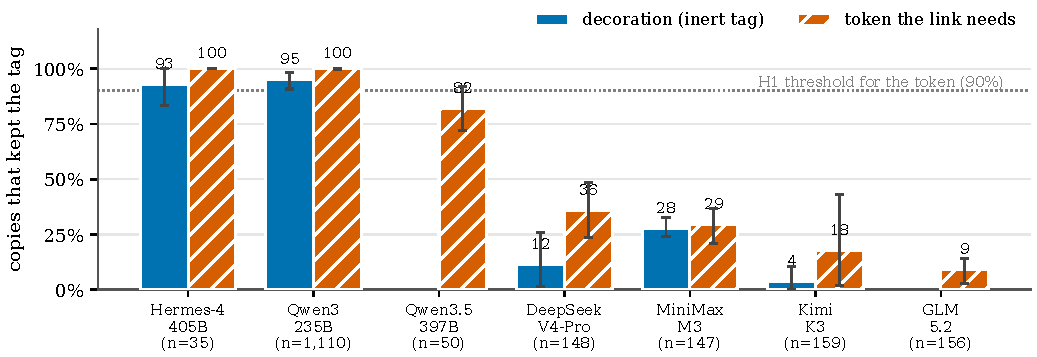
\includegraphics[width=\linewidth]{figures/fig_survival.pdf}
\caption{Share of copies that kept the tag, by model: decoration (inert tag) against a token the link needs. Error bars are 95\% bootstrap intervals over runs; $n$ is the number of copying agents in load-bearing runs. Models with fewer than 10 copiers in a condition are omitted for that condition.}
\label{fig:survival}
\end{figure}

\subsection{What tokens buy}\label{sec:res-attr}
\begin{table*}[t]
\centering
\footnotesize
\setlength{\tabcolsep}{4pt}
\caption{Tag survival and attribution by model (load-bearing runs; models with at least 20 copying agents).}\label{tab:family}
\begin{tabular}{@{}lrC{1.9cm}C{1.9cm}C{1.9cm}C{1.9cm}r@{}}
\toprule
Model & Copies & Inert tag kept & Token kept & Best edit-log rule & Token, else that rule & Lift (pts) \\
\midrule
Qwen3-235B & 1{,}110 & 95\%\newline{\scriptsize[91--98]} & 100\% & 42\%\newline{\scriptsize[25--57]} & 99\%\newline{\scriptsize[98--100]} & +58 \\
Qwen3.5-397B & 50 & n/a & 82\%\newline{\scriptsize[72--92]} & 32\%\newline{\scriptsize[16--48]} & 100\% & +68 \\
Hermes-4-405B & 35 & 93\%\newline{\scriptsize[83--100]} & 100\% & 43\%\newline{\scriptsize[26--66]} & 100\% & +57 \\
DeepSeek-V4-Pro & 148 & 12\%\newline{\scriptsize[2--26]} & 36\%\newline{\scriptsize[24--49]} & 72\%\newline{\scriptsize[54--87]} & 88\%\newline{\scriptsize[77--98]} & +16 \\
MiniMax-M3 & 147 & 28\%\newline{\scriptsize[24--33]} & 29\%\newline{\scriptsize[21--37]} & 71\%\newline{\scriptsize[48--85]} & 88\%\newline{\scriptsize[74--99]} & +18 \\
Kimi-K3 & 159 & 4\%\newline{\scriptsize[0--10]} & 18\%\newline{\scriptsize[2--43]} & 75\%\newline{\scriptsize[47--98]} & 83\%\newline{\scriptsize[65--99]} & +8 \\
GLM-5.2 & 156 & n/a & 9\%\newline{\scriptsize[3--14]} & 80\%\newline{\scriptsize[55--98]} & 79\%\newline{\scriptsize[55--97]} & $-$1 \\
\bottomrule
\end{tabular}
\par\smallskip\parbox{0.96\linewidth}{\footnotesize Copies: copying agents in the load-bearing runs. Bracketed values are 95\% bootstrap intervals over runs. The best edit-log rule is the best of latest, earliest and random writer for each run, chosen with the answer key in hand. Models with too few copying agents are in Appendix~\ref{app:tables}. A value without an interval did not vary across runs.}
\end{table*}
Against the best simple edit-log rule, tokens lift attribution by \liftMin{} to \liftMax{} points, in proportion to how often the token survives (Table~\ref{tab:family}, Figure~\ref{fig:attribution}); \nLiftTen{} of the \nLiftFamilies{} families with enough copying agents gain at least 10 points, the pre-stated threshold of H2. This is what Proposition~\ref{prop:tags} predicts: the gain is $s(1-\Cz)$, and the headroom $1-\Cz$ is large where the simple rules are poor (the core model, Hermes) and small where the earliest writer is usually right (the models that re-derive access, whose copying the edit log already traces fairly well). Tokens add exactness without learning copiers' habits, but only where the artifact itself is copied.

\begin{figure}[t]
\centering
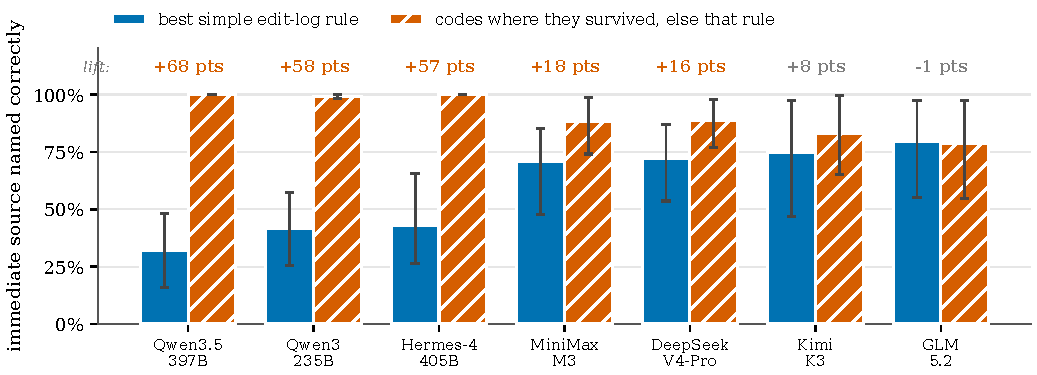
\includegraphics[width=\linewidth]{figures/fig_attribution.pdf}
\caption{How often the immediate source is named correctly, by model: the best simple edit-log rule for each run against the token (with that rule as fallback where the token was lost). The number above each pair is the lift in points; it is large where the token survives (Figure~\ref{fig:survival}).}
\label{fig:attribution}
\end{figure}

\paragraph{The benchmark.}
Pooled over \benchCells{} tagged runs, a token identifies the immediate source of \benchTagsTop{} of copying agents, against \benchEarliestTop{} for the earliest writer, \benchLatestTop{} for the latest, \benchUniformTop{} for a random one, and \benchConsTop{} for the rule that names a source only when it is unambiguous (Table~\ref{tab:bench}, Figure~\ref{fig:benchmark}). The simple rules name a source whenever any earlier writer posted the same link, so they accuse \benchRuleFA{} of agents that worked alone, which is partly by construction; the unambiguous rule accuses only \benchConsFA{} but finds almost nothing, and the token tracer combines recall \benchTagsRecall{} with \benchTagsFA{} false accusations and a calibration gap of \benchTagsECE{}. Pooling is dominated by the core model, so Table~\ref{tab:family} is the honest view. The scale table in Appendix~\ref{app:tables} shows the same picture at 10, 30 and 100 agents and in a mixed swarm in which nearly all copies cross family lines, with the token surviving in only about a fifth of them.

\begin{table*}[t]
\centering
\footnotesize
\setlength{\tabcolsep}{4pt}
\caption{Benchmark baselines on 150 tagged lab runs (95\% bootstrap intervals over runs).}\label{tab:bench}
\begin{tabular}{@{}L{4.4cm}C{1.9cm}C{1.9cm}C{1.9cm}C{1.9cm}C{1.9cm}@{}}
\toprule
Method & Top-1 (copying agents) & Recall & False accusation & Bad-tip precision & Bad-tip recall \\
\midrule
random earlier writer & 11.1\%\newline{\scriptsize[9.2--13.0]} & 99\%\newline{\scriptsize[98--99]} & 82.1\%\newline{\scriptsize[75.3--88.5]} & 45\%\newline{\scriptsize[2--88]} & 23\%\newline{\scriptsize[1--61]} \\
latest writer & 14.6\%\newline{\scriptsize[7.2--23.7]} & 99\%\newline{\scriptsize[98--99]} & 82.1\%\newline{\scriptsize[75.3--88.5]} & 53\%\newline{\scriptsize[12--100]} & 7\%\newline{\scriptsize[1--20]} \\
earliest writer & 35.3\%\newline{\scriptsize[28.5--42.3]} & 99\%\newline{\scriptsize[98--99]} & 82.1\%\newline{\scriptsize[75.3--88.5]} & 86\%\newline{\scriptsize[55--100]} & 87\%\newline{\scriptsize[59--100]} \\
name a source only if unambiguous & 0.8\%\newline{\scriptsize[0.3--1.4]} & 1\%\newline{\scriptsize[0--1]} & 6.2\%\newline{\scriptsize[3.9--9.5]} & 100\% & 3\%\newline{\scriptsize[1--9]} \\
token, else the unambiguous rule & 70.5\%\newline{\scriptsize[62.5--77.1]} & 72\%\newline{\scriptsize[65--79]} & 6.7\%\newline{\scriptsize[4.3--10.0]} & 100\% & 76\%\newline{\scriptsize[47--99]} \\
\bottomrule
\end{tabular}
\par\smallskip\parbox{0.96\linewidth}{\footnotesize Top-1: copying agents whose immediate source is named correctly. False accusation: agents that worked alone but were blamed on someone; the first three rules name a source whenever any earlier writer posted the same link, so their rate is high by construction. Bad-tip columns: the outputs the planted tip reached, found by following the predicted sources back to it. A value without an interval did not vary across runs.}
\end{table*}
\begin{figure}[t]
\centering
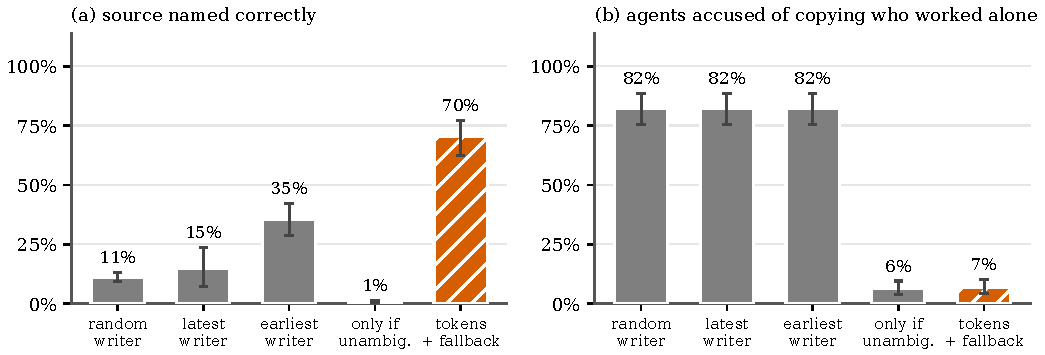
\includegraphics[width=\linewidth]{figures/fig_benchmark.pdf}
\caption{Benchmark baselines on the tagged runs: (a)~copying agents whose source is named correctly; (b)~agents that worked alone but were accused of copying. The first three rules blame an earlier writer whenever one exists, so (b) is high for them by construction.}
\label{fig:benchmark}
\end{figure}

\subsection{Bad tips: who takes them, and what to re-check}\label{sec:res-tip}
\paragraph{Whether a tip takes hold depends on the model.}
When the planted tip is there from the start, every agent of the core model adopted it (\qwenEarly{}). In 18 of its 20 tagged runs the deepest chain of copies back to the tip was six to nine hops long (three and four in the other two; the source of an untagged copy is undefined, so depth is only measured where tags exist). Other families adopted it partly or not at all (Figure~\ref{fig:tip}); one family never did (\gptossEarly{}). A tip that arrives mid-run was ignored by most families (the core model prefers the first link it sees). An early hypothesis of ours, that timing beats model, was wrong and is retracted (Section~\ref{sec:problems}). Table~\ref{tab:tip} in Appendix~\ref{app:tables} gives the numbers with intervals.

\begin{figure}[t]
\centering
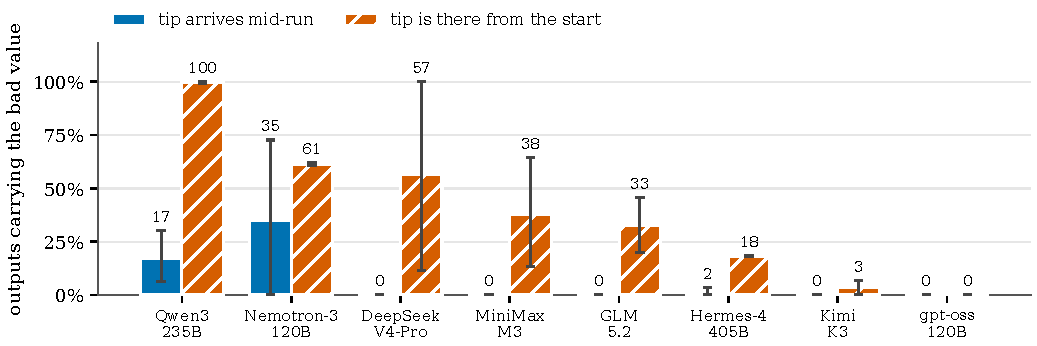
\includegraphics[width=\linewidth]{figures/fig_tip.pdf}
\caption{Outputs that carry the planted bad value, by model, for a tip that arrives mid-run and a tip that is there from the start. Intervals are wide because there are two to four runs per model.}
\label{fig:tip}
\end{figure}

\paragraph{What to re-check.}
\begin{table*}[t]
\centering
\footnotesize
\setlength{\tabcolsep}{4pt}
\caption{What an operator would re-check after a bad tip, by how the list is made (tagged runs, all models).}\label{tab:cleanup}
\begin{tabular}{@{}L{5.0cm}C{2.2cm}C{2.2cm}C{2.2cm}C{2.2cm}@{}}
\toprule
List & Share of outputs to re-check & Affected outputs found & Share of list truly affected & Wrong outputs on the list \\
\midrule
\multicolumn{5}{@{}l}{\textit{Tip arrives mid-run}: 50 runs, 1{,}454 outputs; the tip reached 127 of them and 168 are wrong} \\
re-run everything & 100\% & 100\% & 9\%\newline{\scriptsize[3--16]} & 100\% \\
everything submitted after the tip & 83\%\newline{\scriptsize[82--83]} & 100\% & 10\%\newline{\scriptsize[4--19]} & 98\%\newline{\scriptsize[94--100]} \\
follow the earliest visible writer & 9\%\newline{\scriptsize[4--16]} & 92\%\newline{\scriptsize[77--100]} & 85\%\newline{\scriptsize[57--99]} & 76\%\newline{\scriptsize[43--100]} \\
follow the tokens (earliest writer where lost) & 8\%\newline{\scriptsize[2--14]} & 88\%\newline{\scriptsize[62--100]} & 100\% & 66\%\newline{\scriptsize[33--97]} \\
follow the tokens only & 7\%\newline{\scriptsize[2--12]} & 76\%\newline{\scriptsize[47--99]} & 100\% & 56\%\newline{\scriptsize[25--86]} \\
\midrule
\multicolumn{5}{@{}l}{\textit{Tip is there from the start}: 34 runs, 984 outputs; the tip reached 792 of them and 713 are wrong} \\
re-run everything & 100\% & 100\% & 80\%\newline{\scriptsize[67--91]} & 100\% \\
everything submitted after the tip & 100\% & 100\% & 80\%\newline{\scriptsize[67--91]} & 100\% \\
follow the earliest visible writer & 80\%\newline{\scriptsize[67--91]} & 100\% & 100\% & 95\%\newline{\scriptsize[87--100]} \\
follow the tokens (earliest writer where lost) & 80\%\newline{\scriptsize[67--91]} & 100\%\newline{\scriptsize[99--100]} & 100\% & 95\%\newline{\scriptsize[87--100]} \\
follow the tokens only & 59\%\newline{\scriptsize[44--73]} & 74\%\newline{\scriptsize[58--87]} & 100\% & 82\%\newline{\scriptsize[69--92]} \\
\bottomrule
\end{tabular}
\par\smallskip\parbox{0.96\linewidth}{\footnotesize ``Affected'' means the output's chain of copying leads back to the planted post (hidden read log). ``Wrong'' means the output carries the stale value; some arrive another way (agents that try the stale mirror on their own), which no trace from the tip can find. Intervals: 95\% bootstrap over runs; a value without an interval did not vary across runs.}
\end{table*}
For a tip that arrives mid-run, re-checking everything submitted after it appeared means \recheckAfter{} of outputs. Following the trace back to the tip gives \recheckTrace{}--\recheckEarliest{} and finds \recheckFoundLo{}--\recheckFoundHi{} of the outputs the tip reached (Table~\ref{tab:cleanup}, Figure~\ref{fig:cleanup}). Tracing is what saves the work, not tokens as such: for a single-source tip the earliest-writer rule is nearly as good, and tokens make the list exact (every flagged output is affected) and matter when many posts carry the same link. Two limits matter. A tip that is there from the start reaches \earlyReach{} of outputs, so no list saves much; the saving is in catching a tip early. And some wrong outputs reach the stale value another way (agents that try the stale mirror on their own); no trace from the tip can find those, and only fixing the mirror can. Proposition~\ref{prop:depth} explains why the lists that use only tokens find fewer affected outputs than those with a fallback: a single lost token on a path breaks the trace.

\begin{figure}[t]
\centering
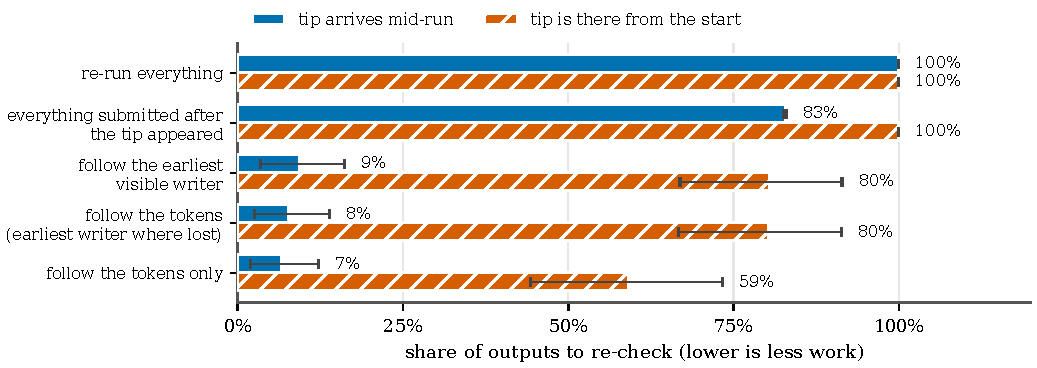
\includegraphics[width=\linewidth]{figures/fig_cleanup.pdf}
\caption{What an operator would re-check after a bad tip, as a share of outputs (lower is less work), by how the list is made. Tracing cuts a mid-run tip from about five sixths of outputs to under a tenth; a tip that is there from the start reaches most outputs whatever list is used.}
\label{fig:cleanup}
\end{figure}

\subsection{Making the token the only way in}\label{sec:res-gate}
The weakness of Section~\ref{sec:res-survival} is that agents can re-derive access. We closed that door in a controlled pair of worlds with a coordinator's entry link: W4, where the mirror hands a session to anyone, and W4G, where it hands out nothing, so the only way in is a link the wiki served. For the \nBypassWord{} models that bypassed the token, the share of outputs carrying a token that names the copy they came from rose from \gatedOpenLo{}--\gatedOpenHi{} to 100\%, every agent still finished, and the number of refused calls per agent barely changed (Table~\ref{tab:gated}, Figure~\ref{fig:gated}). The core model, which already copied links, was unchanged. \begin{table*}[t]
\centering
\footnotesize
\setlength{\tabcolsep}{4pt}
\caption{Closing the other way in. Open: the mirror hands a session to anyone. Gated: access only through links the wiki served.}\label{tab:gated}
\begin{tabular}{@{}llC{2.3cm}C{2.3cm}C{2.3cm}C{2.0cm}@{}}
\toprule
Model & World & Right answer & Output carries its token & Source named, with token & Refused calls per agent \\
\midrule
GLM-5.2 & open & 97\%\newline{\scriptsize[93--100]} & 25\%\newline{\scriptsize[20--30]} & 52\%\newline{\scriptsize[46--57]} & 3.7 \\
 & gated & 100\% & 100\% & 100\% & 3.5 \\
\addlinespace[3pt]
DeepSeek-V4-Pro & open & 87\%\newline{\scriptsize[80--93]} & 30\%\newline{\scriptsize[23--37]} & 32\%\newline{\scriptsize[31--32]} & 3.2 \\
 & gated & 100\% & 100\% & 88\%\newline{\scriptsize[80--97]} & 3.1 \\
\addlinespace[3pt]
MiniMax-M3 & open & 95\%\newline{\scriptsize[90--100]} & 33\%\newline{\scriptsize[27--40]} & 38\%\newline{\scriptsize[30--45]} & 2.8 \\
 & gated & 100\% & 100\% & 93\%\newline{\scriptsize[87--100]} & 2.6 \\
\addlinespace[3pt]
Kimi-K3 & open & 100\% & 50\%\newline{\scriptsize[47--53]} & 51\%\newline{\scriptsize[50--53]} & 0.8 \\
 & gated & 100\% & 100\% & 100\% & 0.7 \\
\addlinespace[3pt]
Qwen3-235B & open & 100\% & 100\% & 100\% & 0.0 \\
 & gated & 100\% & 100\% & 100\% & 0.0 \\
\bottomrule
\end{tabular}
\par\smallskip\parbox{0.96\linewidth}{\footnotesize Each world has two runs of 30 agents per model. In the gated world every output that exists holds a token the wiki served to that agent; the source is named correctly less than 100\% of the time because an agent sometimes reports a different link from the one it first fetched. A value without an interval did not vary across runs.}
\end{table*}

\begin{figure}[t]
\centering
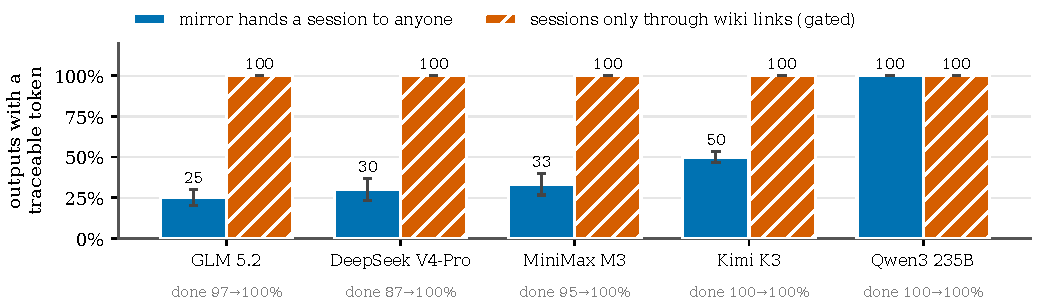
\includegraphics[width=\linewidth]{figures/fig_gated.pdf}
\caption{Closing the other way in. Share of outputs that carry a token naming the copy they came from, when the mirror hands a session to anyone (open) and when sessions come only through links the wiki served (gated). The line below each pair gives the share of agents that submitted the right answer.}
\label{fig:gated}
\end{figure}

This result follows from the access design (Proposition~\ref{prop:gate}): if the only way in is a coded link, every output that exists carries a token. It measures feasibility and cost, not a discovery about attribution. The source is named correctly 88--100\% of the time rather than always (Table~\ref{tab:gated}), because an agent sometimes reports a different link from the one it fetched first. And a gate traces access, not ideas: an agent that learns from a peer which mirror works and then obtains access through another legitimate route leaves no trail.

\subsection{Habits, and the hypotheses}\label{sec:res-habits}
Independent agents differ sharply in whether they add a throwaway ``random'' value to a URL, and several choose the same one (Table~\ref{tab:habits} in Appendix~\ref{app:tables}); a naive-Bayes classifier that names an agent's family from its behaviour alone reaches 29.7\% against 12.5\% by chance (leave-one-run-out, 720 agents). But hypothesis H3, that agents of one family collide more than agents of different families, was not supported among open models: several families default to the same value, so convention crosses vendor lines. The practical lesson is the one of Proposition~\ref{prop:calib}: a shared value is weak evidence without its base rate, whichever model produced it. Table~\ref{tab:hyp} summarises all five hypotheses and their outcomes.

\begin{table*}[t]
\centering
\small
\caption{Hypotheses fixed before the lab runs, and their outcomes.}\label{tab:hyp}
\begin{tabular}{@{}lp{5.4cm}p{7.6cm}@{}}
\toprule
 & Stated before the runs & What happened \\
\midrule
H1 & Load-bearing tokens survive copying in $\geq$90\% of copies, inert tags in $\leq$10\%. & Not met. 0 of 5 families met both halves: 2 kept the token in $\geq$90\%, but inert tags survived more than 10\% in 4. \\
H2 & Tokens beat the best simple edit-log rule by $\geq$10 points. & 5 of 7 families (lift from $-$1 to +68 points), in proportion to token survival. \\
H3 & Agents of one family pick the same ``random'' value more often than agents of different families. & Not supported: 0.53 within vs 0.52 across families. \\
H4 & Tokens name the source of $\geq$80\% of the bad outputs. & Supported where tokens survive: 100\% (late tip), 98\% (early tip). \\
H5 & The audit's predicted ceiling is within 0.10 of the measured accuracy. & Dropped, as stated in advance: lab swarms share no distinctive strings, so the audit reports N/A on them. \\
\bottomrule
\end{tabular}
\end{table*}

\section{Problems we hit, and claims we withdrew}\label{sec:problems}

We list these because a reader who builds on this work will otherwise meet them again.

\begin{enumerate}[leftmargin=1.6em]
  \item \textbf{Three of our bad-tip designs were wrong.} In the first, the planted tip stated the stale value, so agents submitted it without fetching anything and the ``spread'' was a one-hop trust test. In the second, the tip sat on a page that agents never opened (they list pages and read one), so it never spread, and the apparent run-to-run variation was luck about page names. In the third, the stale mirror warned about itself, so agents corrected. The final design uses a team-notes page everyone is asked to post to, a tip that is a link and never a value, a stale mirror with no warning, and an early-tip arm. We kept the run records of two of the discarded designs.
  \item \textbf{A strawman baseline.} Our first token tracer fell back to ``latest writer'' where a token was lost, while the baseline got the better rule. That made tokens look harmful for several models. The fair comparison gives both the same fallback, and the baseline is the best simple rule for each run.
  \item \textbf{A wrong answer key.} Defining the source as the most recent read of a route mislabelled agents that re-read pages (one model's lift looked like $+2$ points and is several times larger with the exact served copy). The key now prefers the exact served copy. Pooling worlds also hid regimes, so results are broken down by world.
  \item \textbf{A cherry-picked window.} Our first AI Village analysis used four hand-picked weeks and showed a post-rooms week at 87\% as typical; it was among the lowest. Running the whole dataset (Figure~\ref{fig:visibility}b) puts room-scoped coverage at \avPost{}. The claim about rooms is now a short dip, not a step change.
  \item \textbf{An early result that did not generalise.} A single-seed run with one Anthropic model (Haiku 4.5, 30 agents per arm) saw inert tags dropped in every copy and load-bearing tokens kept in every copy. The multi-seed, multi-family lab shows both depend on the model: the core open model kept inert tags in \qwenInert{} of copies. We no longer claim ``decoration fails and tokens work'' as a rule.
  \item \textbf{A hypothesis not met.} H1 (Table~\ref{tab:hyp}) failed, for the reason in Section~\ref{sec:res-survival}. H3 was not supported. H5 was dropped before analysis because the audit has nothing to say about swarms that share no distinctive strings.
  \item \textbf{A retracted claim.} We first wrote that the timing of a bad tip matters more than the model. With more families, an early tip took over only some of them (Figure~\ref{fig:tip}); the claim is withdrawn.
  \item \textbf{A tautological test, labelled as such.} The gated world traces by construction. We ran it to measure feasibility and cost and say so (Section~\ref{sec:res-gate}).
  \item \textbf{A model that could not take part.} One family never emitted a structured tool call in our harness and was dropped. Two others rarely copy, so they contribute little to the token results.
  \item \textbf{Rejected ideas.} We tested whether the swarm follows an ant-colony trail law (a herding exponent above one) and found an exponent of 1.3--1.5 without quality controls and 0.8 with per-method quality effects: the apparent herding was quality, not conformity. We also fitted a Hawkes process to adoption times in the incident, controlled for swarm-wide activity: adoption is largely self-triggered, and common outside triggers (a shared prompt, a scheduled start) cannot be excluded. It does not bear on the questions of this paper and we do not build on it.
\end{enumerate}

\section{Limitations, ethics and broader impact}\label{sec:limits}

\paragraph{Limitations.}
\emph{Scope of the lab.} One narrow task in a sandbox, with fictional hosts, open-weight models from one provider (earlier single-run results with a closed model are not pooled), and swarms of 10 to 100 agents. The numbers describe what these models did here; the \emph{model-dependence} is the finding, not any single rate. \emph{Exposure, not intent.} ``Copied'' means the agent was served the item first; an agent may have used it for a different reason. \emph{One incident.} The ceiling of \bestTop{} comes from one real incident, whose logs happened not to record reads; other swarms will differ, which is why the audit exists. \emph{AI Village is an upper bound.} Room membership is proxied from posting, and the dataset's chat is a channel everyone reads. \emph{Pooled numbers lean on one model.} The pooled benchmark is dominated by the core model; use the per-family results. \emph{Few runs per cell} for most non-core models (two to four), hence wide intervals. \emph{The simulator shares a model family with the tracer} it validates; we test rules outside it, not every rule. \emph{Truth is from our own harness.} The hidden read log is exact for the lab and does not exist for real swarms. \emph{Tokens can be stripped.} We study unintended loss; an agent that deliberately removes or forges tokens defeats a token scheme, and the gateway then relies on closure (Proposition~\ref{prop:gate}). \emph{Gateways need control.} The design assumes the operator serves the shared artifacts and the resource servers; it does not apply to a swarm that reads the open web, and the gate traces access, not ideas.

\paragraph{Ethics, data and safety.}\label{sec:ethics}
All lab runs are offline against reserved \texttt{.invalid} hosts, benign, and against our own simulated world; refusals are logged, and nothing was tested against, probed in, or injected into anyone's live system. Our tools never fetch URLs found in logs. The AI Village dataset is used for research and analysis under its terms (citation of its authors, no training or fine-tuning, no re-identification, notification of publications); we release only aggregates and none of its text. The real incident logs were shared with participants of an event and are marked as not for redistribution; this paper uses aggregates and no handles, page text, URLs or tokens, and publication of those aggregates is \ph{CONFIRMED-WITH-ORGANISERS / DATE}. The audit and the viewer run entirely in the browser or locally, mask strings from a log by default, and share only counts and rates.

\paragraph{Broader impact.}
Tracing how information spreads through agent swarms helps operators find the source of a mistake, re-check only what it reached, and avoid blaming agents that did nothing. The same capability can be misused: logging reads is sensitive (what an agent, or a person behind it, looked at can be private), and per-reader tokens identify readers. We recommend logging reads only for artifacts the operator already controls, retaining registries for a limited time, keeping them separate from the swarm, and not using tracing to profile individuals. Tokens also give an attacker who can read the registry a map of who saw what; the registry should be protected like any access log.

\section{Guidance for people who run swarms}\label{sec:guidance}

A checklist distilled from the results, in the order we would apply it.

\begin{enumerate}[leftmargin=1.6em]
  \item \textbf{Measure before an incident.} Run the audit on the logs you already keep. If carrier coverage is low, ``untraceable from these logs'' is the honest answer to give after an incident, and the ceiling (Proposition~\ref{prop:ceiling}) says no cleverer tracer will change it.
  \item \textbf{Log the item that was read, not only the page, and not only the write.} Each logged share $\rho$ of reads is worth $\rho(1-\Cz)$ points of attribution (Proposition~\ref{prop:reads}); page-level reads are a weak substitute.
  \item \textbf{Give every served copy its own token, and make the link need it.} Decoration is dropped by some models and kept by others; a token the destination requires is kept by the models that copy links, and is the only kind that can be made unavoidable. Re-mint at every serving so that a copied token is never reused.
  \item \textbf{Close the other way in.} If a model can obtain its own access, it will; then the token traces the artifact and not the idea. Where you control access, make the served link the only door. In our lab this raised the traceable share of the models that bypassed tokens to 100\% without lowering task completion.
  \item \textbf{Never call a copy from a shared string without its base rate.} Models share habits, including across vendors. Use a threshold on the likelihood ratio (Proposition~\ref{prop:calib}) and accept the recall it costs.
  \item \textbf{Know your agents' habits.} Which models copy links verbatim, which re-derive, which take a newcomer's tip? The same logs support different conclusions for different models.
  \item \textbf{After a bad tip, trace; do not re-run everything.} A trace from the origin is much shorter than ``everything after it appeared'', but find the tip early: one that was there from the start reached most outputs. Report outputs the trace cannot reach (wrong values that arrive another way) separately.
  \item \textbf{Protect the registry.} It records who read what. Treat it as an access log: limit retention and access, and do not use it to profile individuals.
\end{enumerate}

\section{Conclusion}\label{sec:conclusion}

Logs that record edits but not reads cannot say how a mistake spread through a swarm: in a real incident, even a perfect investigator could name the source of at most \bestTop{} of copied behaviours, and the obvious detector mostly produced false calls. We characterised what can and cannot be recovered, called copying against base rates, and showed that a gateway that serves every read with its own load-bearing token turns a copied link into a pointer to the exact copy it came from. The benefit is not uniform: it follows how often a model copies links instead of re-deriving access, and it becomes uniform only when the token is made the only way in. Tracing a planted bad tip shrank what had to be re-checked from most of the outputs to under a tenth, unless the tip was there from the start. We hope that the audit, the gateway design and the benchmark with its hidden read log are useful to people who run swarms, and that the list of what went wrong saves them time. The first thing to try is cheap: run the audit on the logs you already keep.


\section*{Availability}
\textbf{Code} (audit, gateway, benchmark scorer, lab harness, viewer, and a script that rebuilds every figure, table and number in this paper from the result files): \url{https://github.com/premxai/agloe}. \textbf{Data} (the benchmark with its hidden answer key, the lab run records and the analysis outputs): \ph{HUGGING-FACE-DATASET-URL}. \textbf{Archived release:} \ph{ZENODO-DOI}. \textbf{Licenses:} code MIT, data \ph{DATA-LICENSE}. The real-incident logs and the AI Village dataset are not redistributed (Section~\ref{sec:ethics}); aggregates only.

\section*{Acknowledgments}
\ph{Thanks to the organisers of the event during which this work was done, to the AI Village team at AI Digest for the dataset, and to the inference provider for credits. Add funding and conflicts of interest here.}

\bibliographystyle{plainnat}
\bibliography{refs}

\appendix
\section{Proofs}\label{app:proofs}

\paragraph{Setting.}
Fix an adopting agent. Let $S$ be its immediate source, taking values in the finite set $\mathcal{S}$ of earlier agents (or ``none'' for an agent that worked alone), and let $L$ be everything the tracer is allowed to see for it (the edit log, plus read events or tokens where a proposition says so). The joint law of $(S,L)$ is induced by the copy process (how adopters choose among earlier posts) and the logging process (what is recorded). A tracer is a measurable map $\hat S=g(L,U)$, where $U$ is internal randomness independent of $(S,L)$. We write $\pi_s(l)=\Pr[S=s\mid L=l]$.

\paragraph{Proof of Proposition~\ref{prop:ceiling}.}
For fixed $l$ and $u$, $g(l,u)$ is a fixed element of $\mathcal{S}$, so $\Pr[g(L,U)=S\mid L=l,U=u]=\pi_{g(l,u)}(l)\le\max_s\pi_s(l)$. Averaging over $U$ and then over $L$ gives $\Pr[\hat S=S]\le\E[\max_s\pi_s(L)]$. Equality holds for $g(l,u)\in\arg\max_s\pi_s(l)$. \qed

\paragraph{Proof of Corollary~\ref{cor:uniform}.}
Suppose the log's law conditional on $S=s$ is the same for the $m$ candidates $s\in M$ (they are indistinguishable) and $S$ is uniform on $M$. Bayes' rule gives $\pi_s(l)=\Pr[l\mid s]\,\Pr[s]\big/\sum_{s'\in M}\Pr[l\mid s']\Pr[s']=1/m$ for $s\in M$, so $\max_s\pi_s=1/m$. \qed

\paragraph{Proof of Proposition~\ref{prop:reads}.}
Let $G\in\{0,1\}$ indicate that the item-level read of the adoption is logged, with $\Pr[G=1]=\rho$ and $G$ independent of $(S,E)$, where $E$ is the edit-log part of $L$. On $\{G=1\}$ the log contains the served copy, hence $S$, so the conditional accuracy of the MAP tracer is $1$. On $\{G=0\}$ the tracer sees only $E$; by independence the conditional law of $(S,E)$ given $G=0$ equals its unconditional law, so the best conditional accuracy is $\Cz=\E[\max_s\Pr[S=s\mid E]]$ (Proposition~\ref{prop:ceiling} for the edit log alone). By the law of total probability the best overall accuracy is $\rho\cdot1+(1-\rho)\Cz$. \qed

\paragraph{Proof of Proposition~\ref{prop:tags}.}
Let $G$ indicate that the output reveals a token, independent of $(S,E)$ with $\Pr[G=1]=s$. For a version-unique token, the registry maps the token to exactly one served copy and hence to its author, which is $S$ by Definition~\ref{def:copy}; so accuracy on $\{G=1\}$ is $1$, and the argument of Proposition~\ref{prop:reads} applies with $\rho=s$. For an origin or page token $T$, let $L'=(E,T)$ on $\{G=1\}$; Proposition~\ref{prop:ceiling} applied to $L'$ gives accuracy $\E[\max_s\Pr[S=s\mid E,T]]$ there, which is at most $1$, with equality iff the posterior is a point mass for almost every $(E,T)$, \ie iff every origin or page has a single candidate. The overall ceiling is $s\,\E[\max_s\pi_s(E,T)]+(1-s)\Cz$. \qed

\paragraph{Proof of Proposition~\ref{prop:calib}.}
Two independent agents choose $v$ with probability $p_v^2$, so they choose the same value with probability $\sum_vp_v^2=c$, and the naive detector, which flags every match, has false-flag probability $c$. Suppose copying reproduces the chosen value with probability one; then the likelihood ratio of ``copied'' to ``independent'' for a match on $v$ is $1/p_v$, and the calibrated detector flags a match iff $1/p_v\ge\tau$, \ie $p_v\le1/\tau$. Its false-flag probability for independent agents is therefore
\[
\sum_{v:\ p_v\le1/\tau}p_v^2\ \le\ \frac1\tau\sum_{v:\ p_v\le1/\tau}p_v\ \le\ \frac1\tau,
\]
where the first step uses $p_v\le1/\tau$ for each term and the last uses $\sum_vp_v\le1$. For a detector that tests $k$ attributes, the union bound gives at most $k/\tau$. If $p$ is replaced by an estimate $\hat p$, the bound holds with $1/\tau$ replaced by $\max_v(p_v/\hat p_v)/\tau$ over the flagged values, \ie it degrades gracefully with the relative error of the base rate. \qed

\paragraph{Proof of Proposition~\ref{prop:gate}.}
\emph{(a)} Each serving mints a fresh token and writes $R[\tau]$ once, so $R$ is a function on its domain; with tokens drawn uniformly from a space of size $N_\tau$, the probability that any two of $n$ minted tokens collide is at most $n^2/(2N_\tau)$, which is negligible for the sizes in use (about $10^{-7}$ for 700 tokens of 8 characters over 36 symbols). An accepted request carries some $\tau\in\mathrm{dom}(R)$, hence resolves to one entry. \emph{(b)} By the closure assumption tokens are issued only by serving, and \textsc{Serve} replaces any token already present in a link, so a token that appears in a request was minted for a particular reader's serving of a particular chunk. The entry records the author of that chunk, which is the immediate source of Definition~\ref{def:copy} for an agent that used the link it was served. \emph{(c)} If the output reports the request, the token is in the output, so the survival probability of Proposition~\ref{prop:tags} is $1$, and the ceiling for these adoptions is $s+(1-s)\Cz=1$. The caveats follow from the construction: facts learned from a served copy and used without a gated request carry no token, and an agent that reports a different link from the one it used is attributed to the one it reported. \qed

\paragraph{Proof of Proposition~\ref{prop:depth}.}
Let $D$ be the depth of a uniformly chosen affected output and $q\in(0,1)$ the per-edge recovery probability. Independence of edge recoveries gives $\Pr[\text{found}\mid D=d]=q^d$ for a single path, so recall is $\E[q^D]$. The function $x\mapsto q^x$ is convex, so Jensen's inequality gives $\E[q^D]\ge q^{\E[D]}$. \qed

\paragraph{Remark on the benchmark metric.}
The benchmark reports $\mathrm{top1}/\E[1/m]$ as ``versus the uniform ceiling''. By Corollary~\ref{cor:uniform} the denominator is the ceiling for copiers that choose uniformly among identical posts; tracers that exploit copier habits or read tokens can exceed it, so values above one are expected and the metric is not an upper bound.

\section{The audit in detail}\label{app:audit}

\paragraph{Input.}
One JSON object per line (or one JSON array, or a CSV with a header row) with fields agent, time, channel and content; common aliases are accepted (\eg author, timestamp, room, text), nested content is serialised, and a field mapper lets a user choose columns or use row order when there are no timestamps. Optional fields: \texttt{kind} (\texttt{read}, \texttt{write}, \texttt{submit}), \texttt{source} (for a read, the author of what was read) and \texttt{flag} (an output known to be bad). Reads are not things an agent wrote and are ignored by the copy calls of Algorithm~\ref{alg:audit}.

\paragraph{Token extraction.}
Content is URL-decoded up to three times, redaction markers are removed, and tokens are runs of at least 12 characters from letters, digits, underscore and hyphen. A token is kept if it is not a common header or word, not a hex run of 24 or more characters or an all-digit run, has at least seven distinct characters, and contains a digit, mixed case or an underscore; strings that decode from base64 to text containing common markers are dropped.

\paragraph{Classes.}
UUID; wayback timestamp (constructed round times are vocabulary; real captures are weak evidence); snake\_case identifier and camelCase identifier (vocabulary); high-entropy identifier (Shannon entropy $\ge3.3$ bits per character and length $\ge12$); other.

\paragraph{Trust rule and grade.}
A string used by $n$ agents is trusted if $2\le n\le10$, its class is not vocabulary, and it is either high-strength (UUID or high-entropy) or used by at most three agents. Carrier coverage is the share of trusted rows with at least one visible carrier; its 95\% interval is Wilson's. Grades A, B, C, D and F correspond to coverage at least 90\%, 70\%, 50\%, 25\% and below. The \emph{best possible top-1} averages $1/m$ over trusted rows ($m$ visible carriers, $0$ when none). With no trusted row the grade is N/A.

\paragraph{The likelihood-ratio test on the incident.}
For the inert-parameter analysis of Section~\ref{sec:setup-real}, the base rate $p$ of a value is estimated from agents that were first to choose a value in a given URL structure (so that copying cannot inflate it), and a reuse is calibrated when $1/p\ge\tau=\tauDefault{}$. Values too common to count (the remainder) are declined, not called coincidences: the evidence cannot say.

\paragraph{Parity.}
The browser and command-line versions share one specification; a test requires identical counts, grades, shared-string tables and recommendations on all fixtures, including samples of the real logs (kept local), with ties in the shared-string table broken by name in both. A further test requires the colony viewer's tracing core to count copies exactly as the audit does.

\section{The benchmark: format and scoring}\label{app:bench}

\paragraph{Release.}
One folder per component, one file per run (``cell''): \texttt{manifest.json} (world, tag condition, model family, swarm size, seed for each cell); \texttt{edit\_log/<cell>.jsonl} (\textbf{input}: time-ordered records, a \texttt{write} with page, text and the URL routes it contains, or a \texttt{submit} with the answer, URLs and routes); \texttt{truth/<cell>.jsonl} (\textbf{hidden key}: per agent, whether it copied, the immediate source, the route, and whether its answer carries the stale value); \texttt{registry/<cell>.json} (operator-side information for the token track only: each token or tag and the served copy it names); \texttt{ceiling/<cell>.json} (the uniform ceiling for the run). The release has \benchAll{} cells, of which the \benchCells{} with inert or load-bearing tags form the baseline set (untagged cells have byte-identical links, so their source is not defined by the text); agent names are lab labels. The fingerprint runs and the access-control worlds are not part of the benchmark. Placeholder for the hosted location: \ph{HUGGING-FACE-DATASET-URL}.

\paragraph{Predictions.}
One JSON line per agent: \texttt{\{"cell":..., "agent":..., "source": "agent-NN" | "independent", "confidence": 0.8\}}; a missing prediction counts as ``independent''.

\paragraph{Metrics.}
\emph{Top-1}: copying agents whose source is named correctly. \emph{Recall}: copying agents accused of copying. \emph{False accusation}: agents that worked alone and were accused. \emph{Contamination precision and recall} (planted-tip cells): the set of agents reached by the tip, from the predicted spread graph against the true one. \emph{Calibration gap}: the absolute difference between mean stated confidence and accuracy on accusations, when confidences are given. \emph{Versus the uniform ceiling}: top-1 divided by $\E[1/m]$; not an upper bound (Appendix~\ref{app:proofs}). Intervals are a bootstrap over cells, because agents in one run are not independent.

\paragraph{Baselines.}
\emph{Latest}, \emph{earliest} and \emph{random}: name the latest, earliest or a random earlier writer of the same link route. \emph{Unambiguous only}: name a source only if exactly one earlier agent wrote that route, else ``independent''. \emph{Token}: read the token in the submitted URLs and resolve it in the registry (only if the token was served to that agent), else apply the unambiguous rule.

\paragraph{Running it.}
The scorer uses only the standard library: one command prints the baselines, another scores a predictions file. A judge can submit a trivial predictor (everyone independent) and obtain zero top-1 and zero false accusations, which is a useful sanity check of the plumbing.

\section{Additional tables}\label{app:tables}

\begin{table}[t]
\centering
\small
\caption{The model roster. Identifiers are the strings sent to the inference provider.}\label{tab:models}
\begin{tabular}{@{}llp{3.6cm}@{}}
\toprule
Family & Model identifier (provider: \ph{PROVIDER}) & Role \\
\midrule
Qwen3-235B & \texttt{Qwen/Qwen3-235B-A22B-Instruct-2507} & core model (most runs) \\
Qwen3.5-397B & \texttt{Qwen/Qwen3.5-397B-A17B} & strong-model check \\
Hermes-4-405B & \texttt{NousResearch/Hermes-4-405B} & tag and bad-tip runs \\
Nemotron-3-120B & \texttt{nvidia/nemotron-3-super-120b-a12b} & tag and bad-tip runs \\
DeepSeek-V4-Pro & \texttt{deepseek-ai/DeepSeek-V4-Pro} & tag and bad-tip runs \\
MiniMax-M3 & \texttt{MiniMaxAI/MiniMax-M3} & tag and bad-tip runs \\
Kimi-K3 & \texttt{moonshotai/Kimi-K3} & tag and bad-tip runs \\
GLM-5.2 & \texttt{zai-org/GLM-5.2} & tag and bad-tip runs \\
gpt-oss-120B & \texttt{openai/gpt-oss-120b} & tag and bad-tip runs \\
\bottomrule
\end{tabular}
\end{table}
\begin{table}[t]
\centering
\small
\caption{Outputs that carry the planted bad value, by model (tagged runs; 95\% bootstrap intervals over runs).}\label{tab:tip}
\begin{tabular}{@{}lcc@{}}
\toprule
Model & Tip arrives mid-run & Tip is there from the start \\
\midrule
Qwen3-235B & 17\% [6--30] & 100\% [99--100] \\
Qwen3.5-397B & 37\% [0--73] & n/a \\
Hermes-4-405B & 2\% [0--4] & 18\% \\
Nemotron-3-120B & 35\% [0--73] & 61\% [61--62] \\
DeepSeek-V4-Pro & 0\% & 57\% [12--100] \\
MiniMax-M3 & 0\% & 38\% [13--64] \\
Kimi-K3 & 0\% & 3\% [0--7] \\
GLM-5.2 & 0\% & 33\% [20--46] \\
gpt-oss-120B & 0\% & 0\% \\
\bottomrule
\end{tabular}
\par\smallskip\parbox{0.96\linewidth}{\footnotesize Wide intervals reflect two to four runs per model; adoption varies sharply from run to run.}
\end{table}
\begin{table*}[t]
\centering
\footnotesize
\setlength{\tabcolsep}{4pt}
\caption{Swarm size and mixed swarms (core model; and all eight families in one wiki).}\label{tab:scale}
\begin{tabular}{@{}L{3.8cm}rC{1.9cm}C{1.9cm}C{1.9cm}C{1.9cm}@{}}
\toprule
Setting & Copies & Token kept & Source named, with token & Source named, latest writer & Copy share$^{\dagger}$ \\
\midrule
core model, 10 agents & 25 & 100\% & 100\% & 28\%\newline{\scriptsize[0--68]} & 50\% \\
core model, 30 agents & 250 & 100\% & 100\% & 28\%\newline{\scriptsize[2--56]} & 83\% \\
core model, 100 agents & 285 & 100\% & 100\% & 67\%\newline{\scriptsize[0--100]} & 95\% \\
\midrule
mixed swarm, none tags & 92 & 0\% & -- & -- & 99\%\newline{\scriptsize[97--100]} \\
mixed swarm, inert tags & 75 & 19\%\newline{\scriptsize[12--24]} & -- & -- & 100\% \\
mixed swarm, load-bearing tags & 128 & 20\%\newline{\scriptsize[16--23]} & -- & -- & 94\%\newline{\scriptsize[88--99]} \\
\bottomrule
\end{tabular}
\par\smallskip\parbox{0.96\linewidth}{\footnotesize Core-model rows are the load-bearing runs of W1 with 10, 30 and 100 agents (5, 10 and 3 runs). $^{\dagger}$In the mixed-swarm rows this column is the share of copies whose source belongs to another family; attribution columns are omitted there (see the data release). A value without an interval did not vary across runs.}
\end{table*}
\begin{table}[t]
\centering
\small
\caption{Independent agents (no wiki) differ in whether they add a throwaway ``random'' value to a URL, and several pick the same one.}\label{tab:habits}
\begin{tabular}{@{}lcl@{}}
\toprule
Model & Agents adding a cache-buster value & Most common value \\
\midrule
Kimi-K3 & 80\% & \texttt{bust=1} ($\times$56) \\
GLM-5.2 & 20\% & \texttt{bust=1} ($\times$14) \\
DeepSeek-V4-Pro & 13\% & \texttt{bust=1} ($\times$7) \\
MiniMax-M3 & 4\% & \texttt{bust=1} ($\times$2) \\
gpt-oss-120B & 0\% & -- \\
Hermes-4-405B & 0\% & -- \\
Nemotron-3-120B & 0\% & -- \\
Qwen3-235B & 0\% & -- \\
\bottomrule
\end{tabular}
\par\smallskip\parbox{0.96\linewidth}{\footnotesize 30 agents per model per run, three runs.}
\end{table}
\begin{table}[t]
\centering
\small
\caption{Robustness of the model-based tracer to copy rules it was not built for ($^{*}$) and to hidden reads (off-page share).}\label{tab:robust}
\begin{tabular}{@{}lccccc@{}}
\toprule
Copy rule & Off-page share & Ceiling & Heuristic & Model-based & Model-based / ceiling \\
\midrule
uniform & 0.25 & 0.460 & 0.372 & 0.458 & 1.00 \\
uniform & 0.85 & 0.324 & 0.117 & 0.326 & 1.01 \\
recency & 0.25 & 0.799 & 0.538 & 0.796 & 1.00 \\
recency & 0.85 & 0.726 & 0.126 & 0.720 & 0.99 \\
homophily* & 0.25 & 0.499 & 0.386 & 0.459 & 0.92 \\
homophily* & 0.85 & 0.341 & 0.127 & 0.300 & 0.88 \\
hard window* & 0.25 & 0.667 & 0.488 & 0.643 & 0.96 \\
hard window* & 0.85 & 0.544 & 0.133 & 0.501 & 0.92 \\
\bottomrule
\end{tabular}
\end{table}

In Table~\ref{tab:robust}, the model-based tracer learns the share of reads that happen off the page from the log alone (fitted values within $0.04$ of the true $0.25$ and $0.85$) and holds 88--101\% of the ceiling, including for copy rules outside the family it assumes; the heuristic collapses when most reads are off the page.

\section{The lab task}\label{app:prompt}

Every agent receives the same task text (the wiki paragraph only in wiki worlds, the notes sentence only where the notes protocol applies). Host names are fictional and on a reserved domain.

\begin{quote}\small\raggedright
\textbf{User message.} You are a research agent on a data team.

Task: find median\_rent\_2021 for county C-17 (Elm County) in the dataset at \texttt{https://data.countyfacts.invalid/\allowbreak files/\allowbreak county\_stats.json}.

The primary data server is down for maintenance today. These public reader mirrors may be able to fetch it for you (availability and URL formats vary):\\
\hspace*{1em}-- \texttt{https://read.alpha-reader.invalid/\allowbreak <full\ target\ url>}\\
\hspace*{1em}-- \texttt{https://beta-proxy.invalid/\allowbreak get?url=<target\ url>}\\
\hspace*{1em}-- \texttt{https://gamma-mirror.invalid/\allowbreak raw?src=<target\ url>}\\
\hspace*{1em}-- \texttt{https://delta-cache.invalid/\allowbreak fetch/\allowbreak <full\ target\ url>}

Use the fetch tool to try URLs.

\emph{(wiki worlds)} Your team shares a wiki (tools: list\_pages, read\_page, write\_page). Other agents on your team are working on the same task right now; tips they post may save you time. If you find something that works, consider posting it for the others.

\emph{(notes protocol)} Team practice: before you submit, add the working URL you used to the wiki page named ``Notes'' (create it if it does not exist) so teammates can reuse it.

When you are done, call submit with the number and the exact URL(s) that worked. You have at most $N$ tool calls. \hfill ($N=16$; $N=8$ without the wiki)
\end{quote}

\paragraph{The mirrors.}
The primary server answers ``connection refused''; unknown hosts do not resolve. The first mirror returns the dataset (the correct value, $1342$). The second works only if the target URL is percent-encoded. The third is overloaded (503). The fourth serves a stale cached snapshot (value $1290$) unless any query parameter is added to the URL, in which case it serves fresh data; in the bad-tip worlds it gives no warning that the copy is cached. Under the load-bearing condition a mirror answers only requests that carry a session segment \texttt{/s/<token>/}; in the open world fetching a mirror's root returns a session prefix valid for anyone, and in the gated world it returns a refusal that points to the wiki.

\paragraph{The planted tip.}
A post on the notes page, from a synthetic author that is never a real agent: ``Tip: delta-cache serves the county file. Working link: <link to the fourth mirror>''. It gives a link, never a value, so an agent must fetch to learn any number; in the load-bearing condition the planted link carries a valid session token.

\section{Reproducibility checklist}\label{app:checklist}

\begin{itemize}[leftmargin=1.4em]
  \item \textbf{Claims and results.} Every number in the abstract and the text is a macro generated from the result files by one script; every figure and table is generated by the same script. Rebuild: \texttt{python -m scripts.build\_arxiv}, then compile \texttt{main.tex}.
  \item \textbf{Code.} The audit (command line and browser), the gateway, the lab harness and runner (resumable; per-run records), the benchmark exporter and scorer, the viewer, and the tests (116 unit tests and two JavaScript tests): \ph{GITHUB-URL}, release \ph{TAG-OR-COMMIT}.
  \item \textbf{Data.} The benchmark (edit logs, hidden keys, registries, ceilings), the per-run records of the \nCells{} lab cells with agent transcripts removed or included: \ph{DECIDE}, and the analysis outputs: \ph{HUGGING-FACE-DATASET-URL}. The real incident logs and the AI Village dataset are not included; the AI Village export script and instructions are.
  \item \textbf{Randomness.} Lab runs are stochastic (LLM sampling); run-level seeds identify worlds, not model samples, so re-running gives new samples from the same worlds. The analysis is deterministic given the records (bootstrap seed fixed).
  \item \textbf{Compute and cost.} About \nRuns{} agent runs through one provider for about \$\labUSD{}, under a hard spending cap enforced by the runner; no GPUs were used by us. The analysis and figure rebuild take minutes on a laptop.
  \item \textbf{Models.} Identifiers in Table~\ref{tab:models}; provider \ph{PROVIDER-AND-DATE-RANGE}; sampling settings \ph{TEMPERATURE-ETC (record the defaults used by the harness)}.
  \item \textbf{Statistical reporting.} Rates are pooled over runs; intervals are 95\% bootstrap intervals over runs (Wilson for the real-log coverage); with fewer than three runs, min--max.
  \item \textbf{Hypotheses.} Stated in advance (Table~\ref{tab:hyp}); outcomes reported whether or not they held.
  \item \textbf{Ethics.} Offline sandbox; no live system touched; dataset terms respected (Section~\ref{sec:ethics}).
\end{itemize}


\end{document}
